\documentclass[UTF8]{article}
% 中文支持
\usepackage[UTF8]{ctex}	
% pdf调用 封面
\usepackage{pdfpages}
% color宏包
\usepackage{color}  
% 导入图片
\usepackage{caption}
\usepackage{graphicx, subfig}
% 防止图片乱跑
\usepackage{float}
% 支持数学符号
\usepackage{amsmath}
% 支持代码块
\usepackage{listings}
% pdf加入大纲
\usepackage{hyperref}
% 大纲去红框
\hypersetup{hidelinks,
	colorlinks=true,
	allcolors=black,
	pdfstartview=Fit,
	breaklinks=true
}

% 绘制三线表
\usepackage{booktabs}    
% 消除警告
\usepackage{lmodern}

% 绘图
\usepackage{tikz}
\usetikzlibrary{positioning, shapes.geometric}
\tikzstyle{bag} = [align=center]

% 设置页面的环境,a4纸张大小,左右上下边距信息
\usepackage[a4paper, left=31.8mm, right=31.8mm, top=25.4mm, bottom=25.4mm]{geometry}

% 代码块的基本设置
\lstset{
 breaklines,%自动换行
 columns=fixed,       
 numbers=left,                                        % 在左侧显示行号
 numberstyle=\tiny\color{gray},                       % 设定行号格式
 frame=none,                                          % 不显示背景边框
 backgroundcolor=\color[RGB]{245,245,244},            % 设定背景颜色
 keywordstyle=\color[RGB]{40,40,255},                 % 设定关键字颜色
 numberstyle=\footnotesize\color{darkgray},           
 commentstyle=\it\color[RGB]{0,96,96},                % 设置代码注释的格式
 stringstyle=\rmfamily\slshape\color[RGB]{128,0,0},   % 设置字符串格式
 showstringspaces=false,                              % 不显示字符串中的空格
 language=matlab,                                        % 设置语言
}

% 两图片并排
% \begin{figure}[htbp]
% 	\centering
% 	\begin{minipage}{0.49\linewidth}
% 		\centering
% 		\includegraphics[width=0.9\linewidth]{figure/figure_1.jpg}
% 		\caption{title1}
% 		\label{label1} %文中引用该图片代号
% 	\end{minipage}
% 	%\qquad
% 	\begin{minipage}{0.49\linewidth}
% 		\centering
% 		\includegraphics[width=0.9\linewidth]{figure/figure_3.jpg}
% 		\caption{title2}
% 		\label{label2} %文中引用该图片代号
% 	\end{minipage}
% \end{figure}

% 导入图片
% \begin{figure}[H]
%     \centering % 居中 
%     % 图片文件的相对路径
%     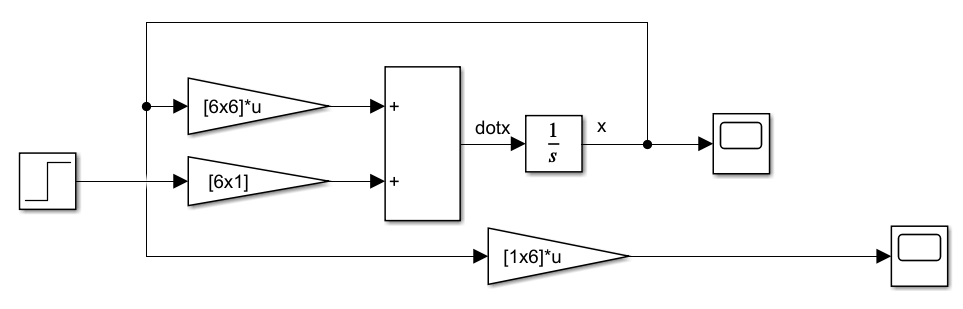
\includegraphics[width=.8\textwidth]{figure/exp1_1_model.png} 
%     \caption{Simulink模型} % caption是图片的标题
%     % \label{img} % 此处的label相当于一个图片的专属标志,目的是方便上下文的引用
% \end{figure}

% 导入代码
% \begin{lstlisting}
% a
% \end{lstlisting}

% 重置章节编号
% \setcounter{section}{0}

% \begin{table}[H] % 防止表格乱跑
% \centering % 居中
% \begin{tabular}{cccccc} % 指明列数
% 	\toprule % 顶部粗线
% 	序号 & 姓名 & 性别 & 年龄 & 身高/cm & 体重/kg \\
% 	\midrule % 中间细线
% 	1 & 张三 & M & 16 & 163 & 50 \\ % 每行末尾都要加换行符
% 	2 & 王红 & F & 15 & 159 & 47 \\
% 	3 & 李二 & M & 17 & 165 & 52 \\
% 	\bottomrule % 底部粗线
% \end{tabular}
% \caption{title} % 标题
% \end{table}

% \begin{thebibliography}{99}  
% 	\bibitem{ref1} 《现场总线技术及应用教程(第二版)》,王永华,机械工业出版社
%   \bibitem{ref13} \href{https://www.elecfans.com/kongzhijishu/1080520.html}{工业控制系统未来的发展趋势分析}:https://www.elecfans.com/kongzhijishu/1080520.html
% \end{thebibliography}

\begin{document}

\begin{titlepage}
% 封面信息

\includepdf[pages={1}]{./cover/cover.pdf}
\end{titlepage}

% 生成目录
\tableofcontents
\cleardoublepage

% 内容:要求、原理、源码、结果、分析等

%
\section{课程设计概述}
%%
\subsection{设计目的}
\begin{itemize}
	\item 自动控制原理理论知识的回顾巩固、进一步理解与基本应用;
	\item MATLAB软件辅助系统分析与设计的学习与应用;
	\item 与自动化专业其它专业课程的对接/衔接尝试。
\end{itemize}


%%
\subsection{设计内容}
\begin{itemize}
	\item 任务一:单级倒立摆系统的建模、分析、设计、验证、半实物平台验证(选);
	\item 任务二:蔡氏混沌电路的建模、分析、同步设计、应用、实现。
\end{itemize}


%%
\subsection{参考资料}
\begin{itemize}
	\item 自动控制原理I和II相关教材;
	\item 相关学术网站(知网)、搜索网站(百度)、MATLAB帮助文件等。
\end{itemize}


%
\section{设计一:单级倒立摆系统}
%%
\subsection{任务概述}
%%%
\paragraph{系统模型建立}~{}
\begin{itemize}
	\item 建立机理非线性模型的状态空间模型和结构图模型;
	\item 建立简化线性模型的状态空间模型、传递函数模型及对应的结构图模型。
\end{itemize}

%%%
\paragraph{开环系统分析}~{}
\begin{itemize}
	\item 分析系统响应:绘制并比较各结构图模型的响应曲线;
	\item 分析简化线性模型的稳定性和性能:基于经典控制方法分析传递函数模型,基于现代控制方法分析状态空间模型;
	\item 分析简化线性模型的能控/能观性:基于现代控制方法,分析状态空间模型的能控/能观性。
\end{itemize}

%%%
\paragraph{系统设计及验证}~{}
\begin{itemize}
	\item 分别设计状态反馈控制器SF、基于状态观测器的状态反馈控制器OSF,实现摆杆出现小偏差后复位;
	\item 设计基于单位比例增益输出反馈的SF/OSF控制器、带积分校正输出反馈的SF/OSF控制器,实现摆杆从A点到B点平衡,分析闭环系统的稳定性和动态性能;
	\item 验证并比较控制器的控制效果。
\end{itemize}


%%
\subsection{系统模型}
%%%
\subsubsection{情境假设}
如下图所示,倒立摆安装在一个小车上,重心处于倒立摆末端。外界可对小车施加水平作用力$u$实施控制,且可以测得小车位移$z$。模型不考虑摆杆质量、摩擦力和风力等作用的影响。具体参数及其取值见下表。
\begin{figure}[htbp]
	\centering
	\begin{minipage}{0.49\linewidth}
		\centering
		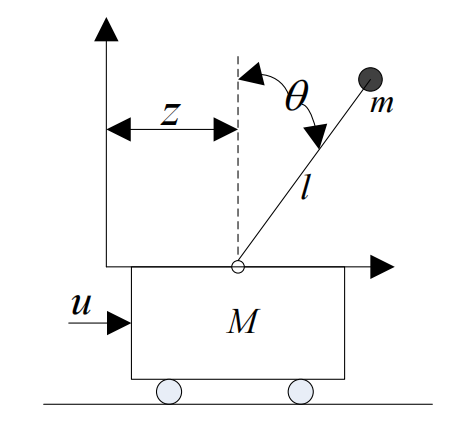
\includegraphics[width=0.9\linewidth]{figure/倒立摆-小车模型.png}
		\caption{倒立摆小车模型}
		% \label{label1} %文中引用该图片代号
	\end{minipage}
	%\qquad
	\begin{minipage}{0.49\linewidth}
		\begin{table}[H] % 防止表格乱跑
		\centering % 居中
		\begin{tabular}{ccc} % 指明列数
			\toprule % 顶部粗线
			参数 & 符号(单位) & 取值 \\
			\midrule % 中间细线
			小车质量 & M($Kg$) & 1.0 \\
			小球质量 & m($Kg$) & 0.1 \\
			摆杆长度 & l($m$) & 0.5 \\
			重力加速度 & g($m/s^2$) & 9.8 \\
			摆杆垂直偏角 & $\theta$($^\circ$) & \textbackslash{} \\
			水平作用力 & u($N$) & \textbackslash{} \\
			\bottomrule % 底部粗线
		\end{tabular}
		\caption{模型参数及取值} % 标题
		\end{table}
	\end{minipage}
\end{figure}

%%%
\subsubsection{机理非线性模型的建立}
对于倒立摆系统,根据牛顿第二定律,可以用如下方程进行描述:

\noindent 在水平方向对摆杆进行受力分析:
\begin{equation*}
	f_w = m\frac{d^2}{dt^2}(z + l\sin\theta) 
\end{equation*}

在竖直方向对摆杆进行受力分析:
\begin{equation*}
	f_v - mg = m\frac{d^2}{dt^2}(l\cos\theta) 
\end{equation*}

由牛顿第二定律在转动情形下的描述,摆杆的合外力矩等于角动量的变化率:
\begin{equation*}
	f_v l\sin\theta - f_w l\cos\theta = J\frac{d^2\theta}{dt^2} \approx 0
\end{equation*}

将小车作为一个整体,进行受力分析,可以得到:
\begin{equation*}
	u - f_w = M\frac{d^2z}{dt^2}
\end{equation*}

对上述各式进行整理,可以得到:
\begin{equation*}
	(\frac{d^2}{dt^2}(l\cos\theta) + g)\sin\theta = (\frac{d^2}{dt^2}(z + l\sin\theta)\cos\theta)
\end{equation*}
\begin{equation*}
	u = m\frac{d^2}{dt^2}(z + l\sin\theta) + M\frac{d^2z}{dt^2}
\end{equation*}

对于倒立摆系统,定义如下状态分量:
\begin{equation*}
	\begin{bmatrix}
		x_1 \\
		x_2 \\
		x_3 \\
		x_4 \\
	\end{bmatrix} = 
	\begin{bmatrix}
		z \\
		\dot{z} \\
		\theta \\
		\dot{\theta} \\
	\end{bmatrix}
\end{equation*}

将以上状态分量代入方程,经过整理即可得到机理非线性模型的状态空间表达式,如下所示:
\begin{equation*}
	\begin{bmatrix}
		\dot{x}_1 \\
		\dot{x}_2 \\
		\dot{x}_3 \\
		\dot{x}_4 \\
	\end{bmatrix} = 
	\begin{bmatrix}
		x_2 \\
		\frac{u + mlx_4^2\sin x_3 - mg\sin x_3 \cos x_3}{M + m - m\cos^2x_3} \\
		x_4 \\
		\frac{-u\cos x_3 + (M + m)g\sin x_3 - mlx_4^2\sin x_3\cos x_3}{(M + m)l - ml\cos^2x_3} 
	\end{bmatrix}
\end{equation*}

%%%
\subsubsection{简化线性模型的建立}
%%%%
\paragraph{状态空间模型}~{}

采用点线性化方法,将倒立摆的机理非线性系统在平衡点$\theta = 0$处进行线性化处理。由于$\theta$非常小,可以做如下的近似处理:
\begin{equation*}
	\sin x_3 \approx x_3 \approx 0 
\end{equation*}
\begin{equation*}
	\cos x_3 \approx 1 
\end{equation*}

定义系统输出为$y = z$,结合上述处理即可将非线性模型转为线性模型:
\begin{equation*}
	\begin{bmatrix}
		\dot{x}_1 \\
		\dot{x}_2 \\
		\dot{x}_3 \\
		\dot{x}_4 \\
	\end{bmatrix} = 
	\begin{bmatrix}
		x_2 \\
		\frac{u - mgx_3}{M} \\
		x_4 \\
		\frac{-u + (M + m)gx_3}{Ml} \\
	\end{bmatrix} = 
	\begin{bmatrix}
		0 & 1 & 0 & 0 \\
		0 & 0 & \frac{-mg}{M} & 0 \\
		0 & 0 & 0 & 1 \\
		0 & 0 & \frac{(M + m)g}{Ml} & 0 \\
	\end{bmatrix}
	\begin{bmatrix}
		x_1 \\
		x_2 \\
		x_3 \\
		x_4 \\
	\end{bmatrix} + 
	\begin{bmatrix}
		0 \\
		\frac{1}{M} \\
		0 \\
		\frac{-1}{Ml}
	\end{bmatrix}u
\end{equation*}
\begin{equation*}
	y = x_1 = [1 \quad 0 \quad 0 \quad 0]x
\end{equation*}

%%%%
\paragraph{传递函数模型}~{}

基于简化线性模型的状态空间表达式,利用MATLAB可以得到其传递函数模型:
\begin{equation*}
	\begin{split}
		G(s) &= \frac{(s + 4.427)(s - 4.427)}{s^2(s - 4.643)(s + 4.643)} \\
		&= \frac{s^2 - 19.6}{s^4 - 21.56s^2} \\
	\end{split}
\end{equation*}

%%
\subsection{系统分析}
%%%
\subsubsection{系统响应分析}
% 设置微小的角度偏差、无控制输入
% 2. 绘制基于非线性系统模型的响应曲线,
% 观察并分析各状态的演变过程
% 3. 绘制基于线性系统模型的响应曲线,观
% 察并分析各状态的演变过程
% 4. 比较两种模型下响应曲线的异同,并分
% 析原因
在simulink中分别搭建非线性模型和线性模型:
\begin{figure}[H]
    \centering % 居中 
    % 图片文件的相对路径
    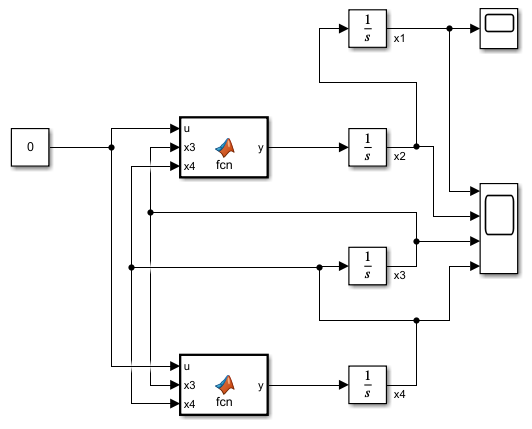
\includegraphics[width=.6\textwidth]{figure/倒立摆-非线性模型.png} 
    \caption{倒立摆非线性模型} % caption是图片的标题
    % \label{img} % 此处的label相当于一个图片的专属标志,目的是方便上下文的引用
\end{figure}
\begin{figure}[H]
    \centering % 居中 
    % 图片文件的相对路径
    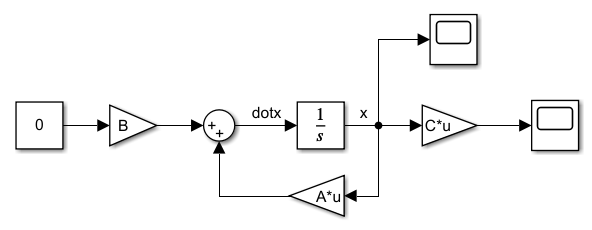
\includegraphics[width=.6\textwidth]{figure/倒立摆-线性模型.png} 
    \caption{倒立摆线性模型} % caption是图片的标题
    % \label{img} % 此处的label相当于一个图片的专属标志,目的是方便上下文的引用
\end{figure}

针对上述两个模型,在无控制输入的情况下,在积分器中设置微小的角度偏差,得到各状态的变化曲线如下所示:
\begin{figure}[H]
    \centering % 居中 
    % 图片文件的相对路径
    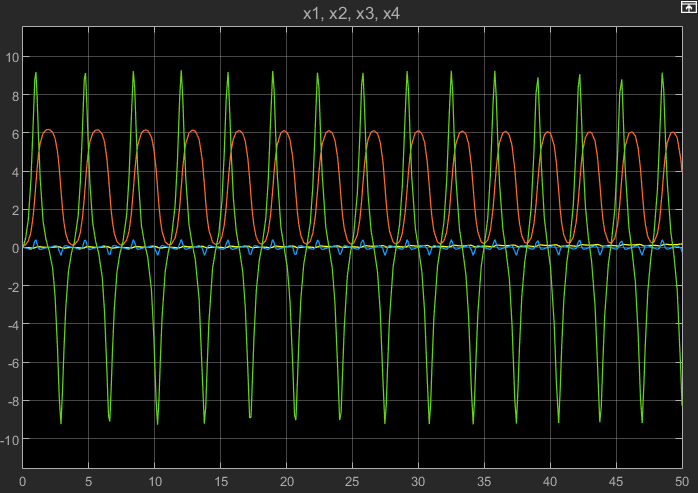
\includegraphics[width=.6\textwidth]{figure/倒立摆-非线性模型-开环响应.png} 
    \caption{非线性模型响应曲线} % caption是图片的标题
    % \label{img} % 此处的label相当于一个图片的专属标志,目的是方便上下文的引用
\end{figure}
\begin{figure}[H]
    \centering % 居中 
    % 图片文件的相对路径
    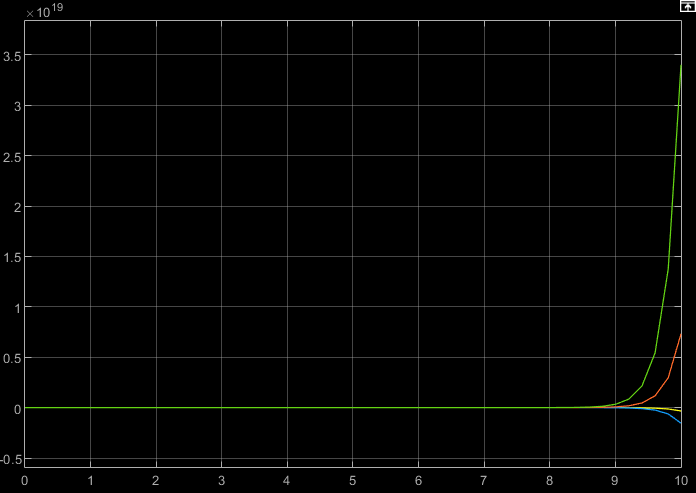
\includegraphics[width=.6\textwidth]{figure/倒立摆-线性模型-开环响应.png} 
    \caption{线性模型响应曲线} % caption是图片的标题
    % \label{img} % 此处的label相当于一个图片的专属标志,目的是方便上下文的引用
\end{figure}
由以上两个响应曲线图可以看出,非线性模型和线性模型都是不稳定的。非线性模型的响应曲线呈现出等幅振荡的形式,而线性模型的响应曲线则在不断发散。

另外,根据线性系统的传递函数模型可以得到系统的阶跃响应曲线,如下图所示:
\begin{figure}[H]
    \centering % 居中 
    % 图片文件的相对路径
    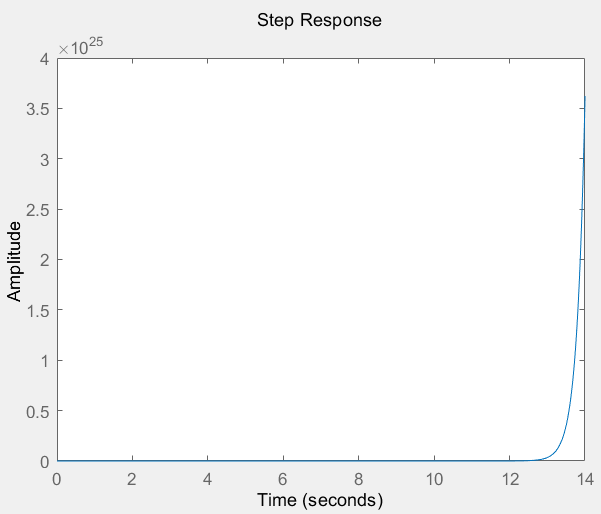
\includegraphics[width=.6\textwidth]{figure/倒立摆-传函-阶跃响应.png} 
    \caption{线性系统传递函数的阶跃响应} % caption是图片的标题
    % \label{img} % 此处的label相当于一个图片的专属标志,目的是方便上下文的引用
\end{figure}
其变化情况与上述线性模型的状态响应曲线一致。

%%%
\subsubsection{系统稳定性与性能分析}
% 1. 基于传递函数模型分析稳定性:极点分布法、Bode图法、Nyquist图法等(选一种)
% 2. 基于传递函数模型分析性能:幅值裕度、相角裕度、截止频率、等
% 3. 基于状态空间模型分析状态稳定性:李氏间接法、李氏直接法
% 4. 对比开环系统响应曲线,验证以上稳定性相关结论的正确性

%%%%
\paragraph{基于传递函数模型的稳定性分析}~{}
\begin{itemize}

\item 极点分布:由线性系统的传递函数模型可以计算得到系统的极点如下:
\begin{equation*}
	\lambda_1 = \lambda_2 = 0,\ \lambda_3 = -4.643,\ \lambda_4 = 4.643
\end{equation*}
系统存在极点位于s右半平面,因此系统是不稳定的。

\item Bode图:根据线性系统传递函数模型,绘制系统Bode图:
\begin{figure}[H]
    \centering % 居中 
    % 图片文件的相对路径
    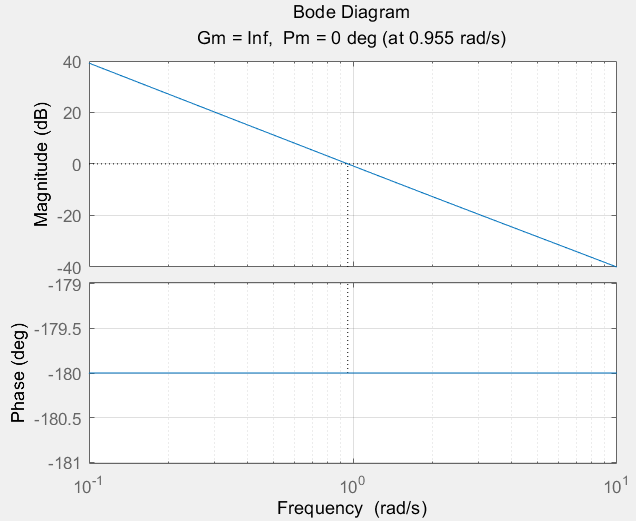
\includegraphics[width=.6\textwidth]{figure/倒立摆-bode图.png} 
    \caption{线性系统Bode图} % caption是图片的标题
    % \label{img} % 此处的label相当于一个图片的专属标志,目的是方便上下文的引用
\end{figure}
对照Bode图分析可知,系统幅值裕度、相角裕度均为零,故系统是不稳定的。

\item Nyquist图:根据线性系统传递函数模型,绘制Nyquist曲线:
\begin{figure}[H]
    \centering % 居中 
    % 图片文件的相对路径
    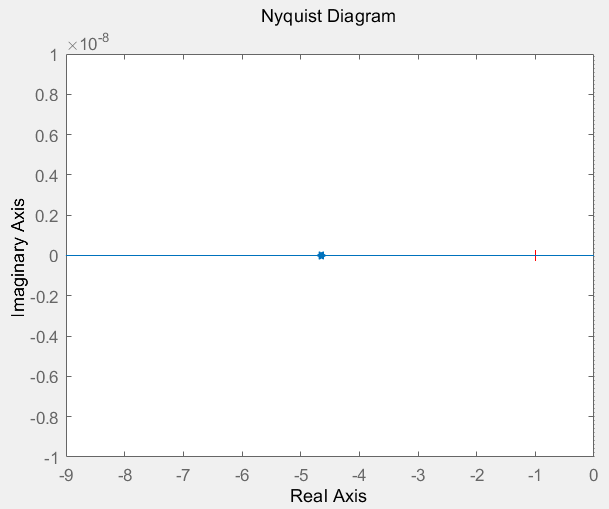
\includegraphics[width=.6\textwidth]{figure/倒立摆-奈氏曲线.png} 
    \caption{线性系统Nyquist图} % caption是图片的标题
    % \label{img} % 此处的label相当于一个图片的专属标志,目的是方便上下文的引用
\end{figure}
由前述系统极点的分布情况,系统在s右半平面的极点数为1,则$P = 1$;由上图可知,系统Nyquist曲线包围$(-1,\ j0)$的圈数为0,则$N = 0$。最终有$Z = P - 2N = 1 \ne 0$,故系统不稳定。

\end{itemize}

%%%%
\paragraph{基于状态空间模型的稳定性分析}~{}

\begin{itemize}

\item 李雅普诺夫第一法:利用系统矩阵A,求得系统的所有特征根:
\begin{equation*}
	\lambda_1 = \lambda_2 = 0,\ \lambda_3 = -4.643,\ \lambda_4 = 4.643
\end{equation*}
系统存在有正实部的特征根,因此系统是不稳定的。

\item 李雅普诺夫第二法:根据李雅普诺夫方程$A^TP + PA = -Q$,在矩阵A,Q给定的情况下,求解出P,则系统为渐进稳定的充要条件为矩阵P为正定矩阵。此处使用LMI方法求解,代码如下:
\begin{lstlisting}
%LMI方法(间接法) 李二判别法
P_SF = sdpvar(4, 4, 'symmetric');
Fcond = [P_SF>=0, A'*P_SF+P_SF*A<=0];%注意严格大于等于
ops = sdpsettings('verbose', 0, 'solver', 'sedumi');%设置求解环境
diagnostics = solvesdp(Fcond, [], ops);%迭代求解
[m, p] = checkset(Fcond);%返回求解结果
tmin = min(m);%验证是否满足
if tmin > 0
    disp('稳定')
else 
    disp('不稳定')
end
\end{lstlisting}
程序运行结果表明,系统是不稳定的。

\end{itemize}

%%%%
\paragraph{性能分析}~{}

对照Bode图可以计算得到系统的幅值裕度、相角裕度、截止频率等,结果如下:
\begin{table}[H] % 防止表格乱跑
\centering % 居中
\begin{tabular}{ccc} % 指明列数
	\toprule % 顶部粗线
	符号 & 说明 & 数值 \\
	\midrule % 中间细线
	$G_m$ & 幅值裕度 & 0 \\
	$P_m$ & 相角裕度 & 0 \\
	$w_c$ & 截止频率 & 0.9554 \\
	$w_g$ & 相角交界频率 & 0 \\
	\bottomrule % 底部粗线
\end{tabular}
\caption{系统频域性能指标} % 标题
\end{table}

%%%
\subsubsection{能控性与能观性分析}

%%%%
\paragraph{秩判据}~{}

利用MATLAB中的能控、能观性判别矩阵计算函数$ctrb(),\ obsv()$,分别计算系统的能控和能观性判别矩阵$Q_c,\ Q_o$如下:
\begin{equation*}
	Q_c = \begin{bmatrix}
		0 & 1 & 0 & 1.96 \\
		1 & 0 & 1.96 & 0 \\
		0 & -2 & 0 & -43.12 \\
		-2 & 0 & -43.12 & 0 \\
	\end{bmatrix},\ 
	Q_o = \begin{bmatrix}
		1 & 0 & 0 & 0 \\
		0 & 1 & 0 & 0 \\
		0 & 0 & -0.98 & 0 \\
		0 & 0 & 0 & -0.98 \\
	\end{bmatrix}
\end{equation*}

容易知道上述能控和能观性判别矩阵均为满秩,故系统是能控且能观的。

%%%%
\paragraph{约旦标准形}~{}

对线性模型的原状态空间表达式做线性变换,将其变换为约旦标准形,约旦块矩阵J及变换后的$\tilde{B},\ \tilde{C}$矩阵如下:
\begin{equation*}
	J = \begin{bmatrix}
		0 & 1 & 0 & 0 \\
		0 & 0 & 0 & 0 \\
		0 & 0 & -4.64 & 0 \\
		0 & 0 & 0 & 4.64 \\
	\end{bmatrix},\ 
	\tilde{B} = \begin{bmatrix}
		0 \\
		0.05 \\
		-1.02 \\
		-1.02 \\
	\end{bmatrix},\ 
	\tilde{C} = \begin{bmatrix}
		0.045 & 0 & 0.005 & -0.005
	\end{bmatrix}
\end{equation*}

分析上述矩阵特点可以知道,约旦块矩阵$J$对应的$\tilde{B}$末尾行非全零,约旦块矩阵$J$对应的$\tilde{C}$首列非全零,故系统是能控且能观的。


%%
\subsection{系统设计与验证}
% 设计状态反馈(SF)控制策略,实现摆杆出现小偏差后复位,即设计镇定控制器

% 设计基于状态观测器的状态反馈(OSF)控制策略,实现摆杆出现小偏差后复位

% 设计控制策略,实现摆杆从A点到B点(可简化看作,跟踪单位阶跃形式的位移信号)
% 在原状态反馈结构基础上,引入输出反馈控制,尝试实现跟踪位移信号
% 在原状态反馈结构基础上,引入带积分校正的输出反馈控制,实现跟踪位移信号

%%%
\subsubsection{任务1:摆杆出现微小偏差后复位(镇定控制器)}
%%%%
\paragraph{状态反馈(SF)}~{}
% 1. 基于极点配置方法和线性模型,设计状态反馈控制器,实现原正常倒立摆杆出现微小角度偏离后复位
% 2. 基于simulink平台验证控制器效果:简化线性系统 + 状态反馈控制器
% 3. 基于simulink平台验证控制器效果:原始非线性系统 + 状态反馈控制器
% 4. 绘制两类闭环系统条件下的响应曲线,比较异同,分析原因

经过前面的分析已经知道,线性系统是完全能控的,因此可以通过状态反馈对该线性系统进行极点的任意配置,以实现系统镇定。此处我们选取闭环系统的极点为:
\begin{equation*}
	P_{sf} = [-1,\ -2,\ -3,\ -4]
\end{equation*}

分别获取状态反馈闭环系统的特征多项式和期望特征多项式,即:
\begin{align*}
	f(\lambda) &= |\lambda I - (A + BK)| \\
	f^*(\lambda) &= \prod_{i=1}^n(\lambda - \lambda^*_i)
\end{align*}

通过对比两者相同次项的系数,求解方程组即可得到状态反馈增益矩阵K。此处我们使用MATLAB提供的$acker()$函数,以获取指定极点配置下的状态反馈增益矩阵K:
\begin{lstlisting}
P_sf = [-1, -2, -3, -4];
% 计算给定极点下的状态反馈增益
% 注意这里的状态反馈增益的符号与书上相反
K_sf = -acker(A, B, P_sf);
\end{lstlisting}
计算结果:
\begin{equation*}
	K_{sf} = [1.224,\ 2.551,\ 28.892,\ 6.276]
\end{equation*}

在simulink中分别搭建非线性和线性模型的状态反馈结构图:
\begin{figure}[H]
    \centering % 居中 
    % 图片文件的相对路径
    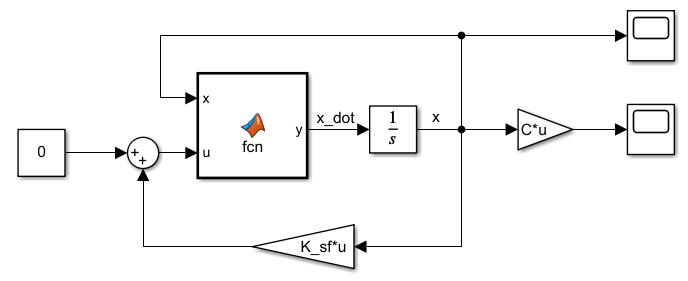
\includegraphics[width=.6\textwidth]{figure/倒立摆-非线性模型-状态反馈.png} 
    \caption{非线性模型状态反馈结构图} % caption是图片的标题
    % \label{img} % 此处的label相当于一个图片的专属标志,目的是方便上下文的引用
\end{figure}
\begin{figure}[H]
    \centering % 居中 
    % 图片文件的相对路径
    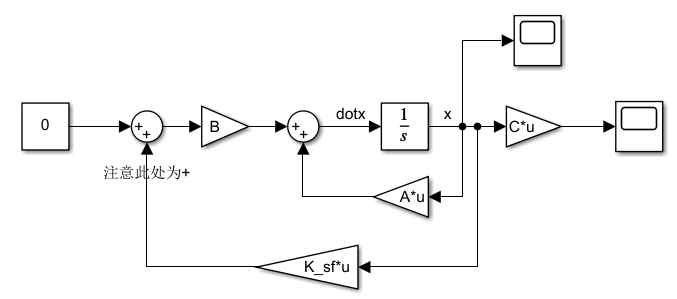
\includegraphics[width=.6\textwidth]{figure/倒立摆-线性模型-状态反馈.png} 
    \caption{线性模型状态反馈结构图} % caption是图片的标题
    % \label{img} % 此处的label相当于一个图片的专属标志,目的是方便上下文的引用
\end{figure}

在初始状态均为$[0,\ 0,\ 1,\ 0]$,输入为零的条件下,即在初始时刻设定一个微小的角度偏差,得到的系统响应曲线分别如下所示:
\begin{figure}[H]
    \centering % 居中 
    % 图片文件的相对路径
    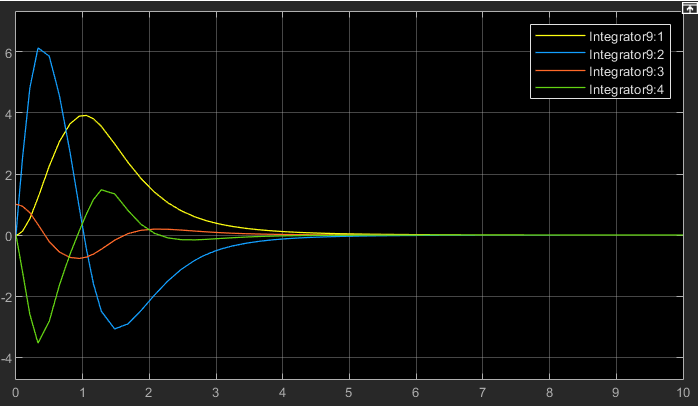
\includegraphics[width=.6\textwidth]{figure/倒立摆-非线性模型-状态反馈-响应曲线.png} 
    \caption{非线性模型状态反馈响应曲线} % caption是图片的标题
    % \label{img} % 此处的label相当于一个图片的专属标志,目的是方便上下文的引用
\end{figure}
\begin{figure}[H]
    \centering % 居中 
    % 图片文件的相对路径
    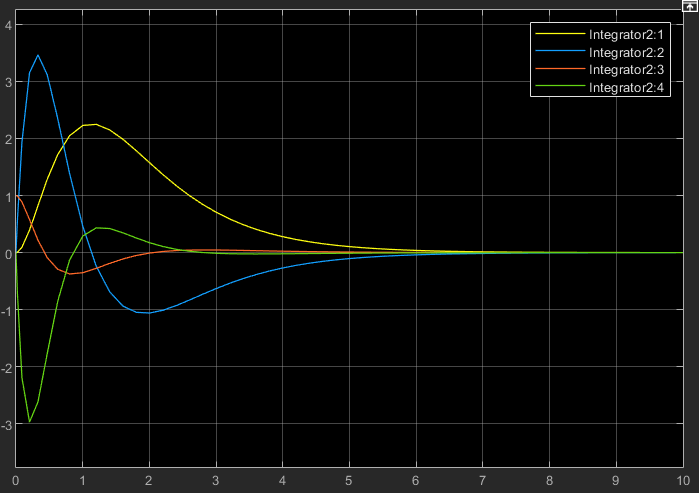
\includegraphics[width=.6\textwidth]{figure/倒立摆-线性模型-状态反馈-响应曲线.png} 
    \caption{线性模型状态反馈响应曲线} % caption是图片的标题
    % \label{img} % 此处的label相当于一个图片的专属标志,目的是方便上下文的引用
\end{figure}

通过对比上述非线性与线性模型的响应曲线可以发现,两者的响应变化情况基本一致。

%%%%
\paragraph{基于状态观测器的状态反馈(OSF)}~{}

% 1. 基于极点配置方法和线性模型,设计基于状态观测器的状态反馈控制策略,实
% 现原正常倒立摆杆出现微小角度偏离后复位
% 2. 基于Simulink平台验证控制器效果:简化线性系统 + SF控制器或OSF控制器
% 3. 基于Simulink平台验证控制器效果:原始非线性系统 + SF控制器或OSF控制器
% 4. 绘制四类闭环系统条件下的响应曲线,比较异同,分析原因
指定状态观测器的极点配置为$P_osf = [-1,\ -2,\ -3,\ -4]$,通过函数$acker()$求解观测器状态反馈矩阵G:
\begin{lstlisting}
P_osf = [-1, -2, -3, -4];
% 计算给定极点下的状态观测器输出误差反馈矩阵
G = (acker(A', C', P_osf))';
\end{lstlisting}
计算结果:
\begin{equation*}
	G = \begin{bmatrix}
		10.000 \\
		56.560 \\
		-271.020 \\
		-1268.810
	\end{bmatrix}
\end{equation*}

在simulink中分别搭建非线性和线性模型的基于状态观测器的状态反馈结构图:
\begin{figure}[H]
    \centering % 居中 
    % 图片文件的相对路径
    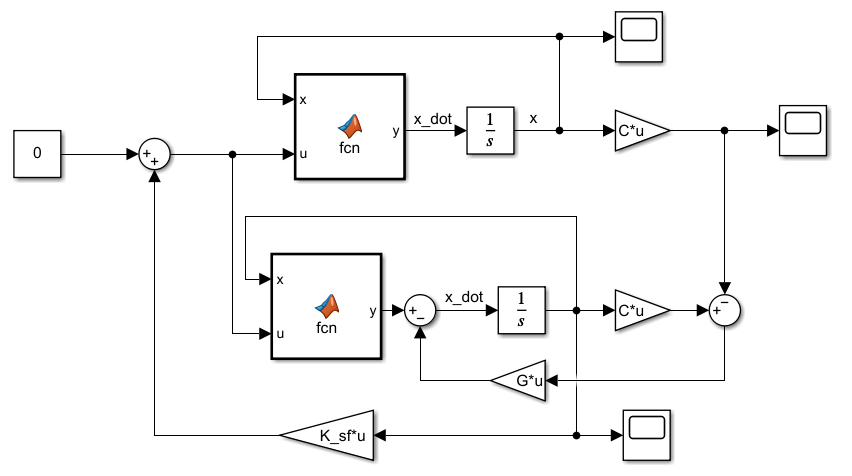
\includegraphics[width=.6\textwidth]{figure/倒立摆-非线性模型-状态观测器.png} 
    \caption{非线性模型基于状态观测器的状态反馈} % caption是图片的标题
    % \label{img} % 此处的label相当于一个图片的专属标志,目的是方便上下文的引用
\end{figure}
\begin{figure}[H]
    \centering % 居中 
    % 图片文件的相对路径
    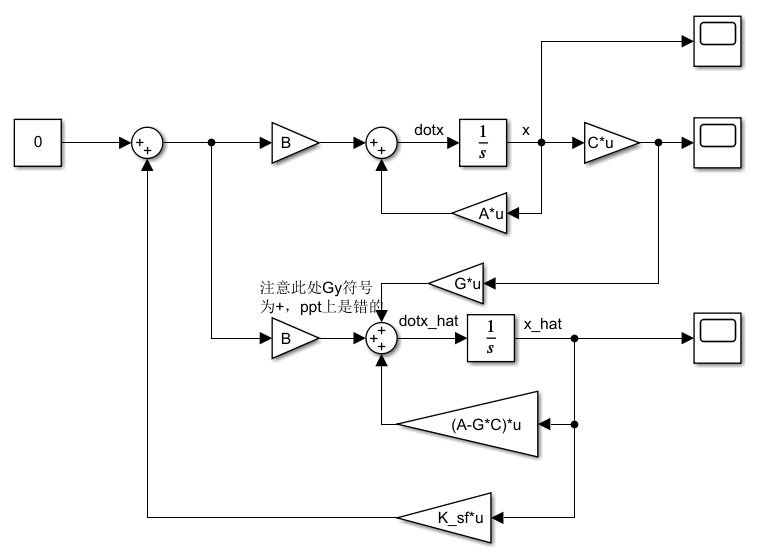
\includegraphics[width=.6\textwidth]{figure/倒立摆-线性模型-状态观测器.png} 
    \caption{线性模型基于状态观测器的状态反馈} % caption是图片的标题
    % \label{img} % 此处的label相当于一个图片的专属标志,目的是方便上下文的引用
\end{figure}

在初始状态均为$[0,\ 0,\ 0.1,\ 0]$,输入为零的条件下,即在初始时刻设定一个微小的角度偏差,得到的系统响应曲线分别如下所示:
\begin{figure}[H]
	\centering
	\begin{minipage}{0.49\linewidth}
		\centering
		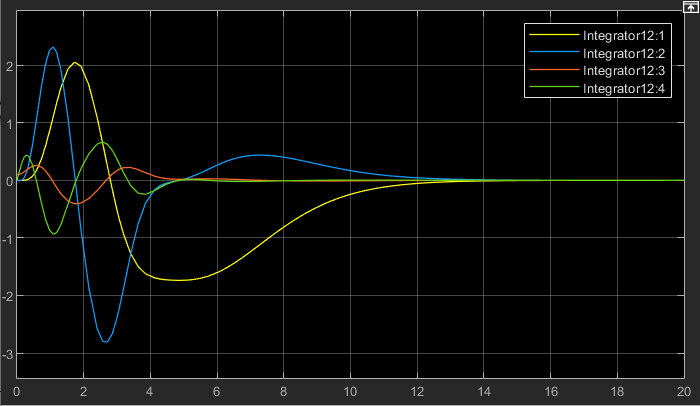
\includegraphics[width=0.9\linewidth]{figure/倒立摆-非线性模型-状态观测器-实际状态.png}
		\caption{非线性模型-实际状态}
		% \label{label1} %文中引用该图片代号
	\end{minipage}
	%\qquad
	\begin{minipage}{0.49\linewidth}
		\centering
		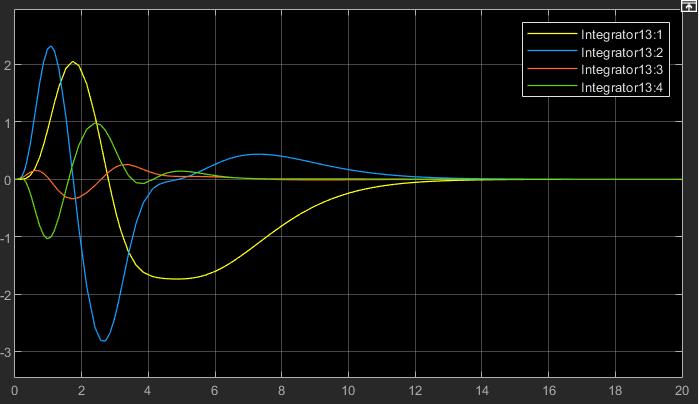
\includegraphics[width=0.9\linewidth]{figure/倒立摆-非线性模型-状态观测器-观测状态.png}
		\caption{非线性模型-观测状态}
		% \label{label2} %文中引用该图片代号
	\end{minipage}
\end{figure}
\begin{figure}[H]
	\centering
	\begin{minipage}{0.49\linewidth}
		\centering
		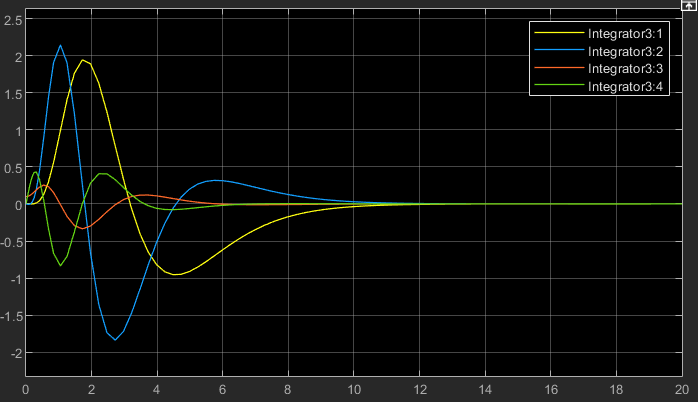
\includegraphics[width=0.9\linewidth]{figure/倒立摆-线性模型-状态观测器-实际状态.png}
		\caption{线性模型-实际状态}
		% \label{label1} %文中引用该图片代号
	\end{minipage}
	%\qquad
	\begin{minipage}{0.49\linewidth}
		\centering
		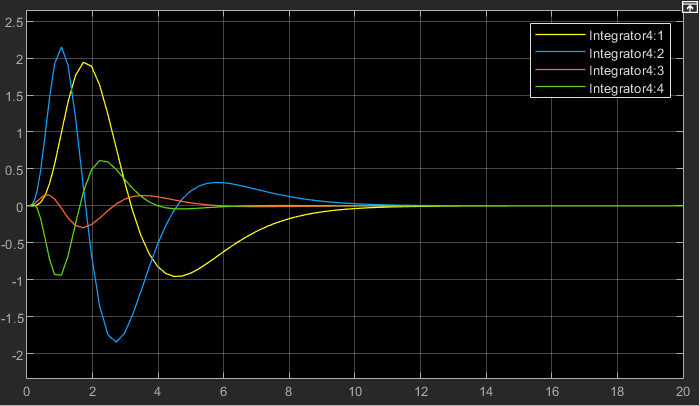
\includegraphics[width=0.9\linewidth]{figure/倒立摆-线性模型-状态观测器-观测状态.png}
		\caption{线性模型-观测状态}
		% \label{label2} %文中引用该图片代号
	\end{minipage}
\end{figure}

对比以上各图容易看出,首先,非线性模型和线性模型的状态观测器的状态观测值输出与实际状态值基本一致,说明状态观测器的设计是合理的;其次,非线性模型与线性模型的状态变化情况非常相近,这说明在原先机理非线性模型的基础上进行简化得到的线性模型是可取的。

%%%
\subsubsection{任务2:实现摆杆从A点到B点(跟踪阶跃位移信号)}
%%%%
\paragraph{基于原状态反馈的单位输出反馈控制}~{}

% 1. 在原状态反馈结构基础上,引入输出反馈控制,尝试实现跟踪位移信号
% 2. 基于极点配置方法和线性模型,设计状态反馈控制器增益K1
% 3. 基于simulink平台验证控制器效果:简化线性系统 + 控制策略
% 4. 基于simulink平台验证控制器效果:原始非线性系统 + 控制策略
% 5. 绘制两类闭环系统的输出响应曲线,比较异同与跟踪效果,分析原因

在原状态反馈结构基础上,引入单位比例的输出反馈,其结构示意如下:
\begin{figure}[H]
    \centering % 居中 
    % 图片文件的相对路径
    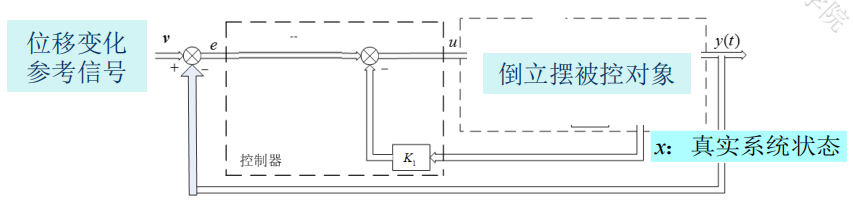
\includegraphics[width=.6\textwidth]{figure/倒立摆-输出反馈示意图.png} 
    \caption{基于原状态反馈的单位输出反馈示意图} % caption是图片的标题
    % \label{img} % 此处的label相当于一个图片的专属标志,目的是方便上下文的引用
\end{figure}
其中,对于状态反馈控制器部分,有如下状态空间表达式:
\begin{equation*}
	\begin{cases}
		\dot{x} = (A + BK_{sf})x + Bu \\
		y = Cx
	\end{cases}
\end{equation*}

引入单位输出反馈控制率:
\begin{equation*}
	u = v - y = v - Cx
\end{equation*}

代入整理得到输出反馈系统的状态空间表达式:
\begin{equation*}
	\begin{cases}
		\dot{x} = [A + B(K_{sf} - C)]x + Bv \\
		y = Cx
		\end{cases}
\end{equation*}

对比原状态反馈控制器的表达式可以看出,它们的形式基本一致,说明该输出反馈系统实际上仍可以转换成一个状态反馈系统,其状态反馈增益矩阵为$K_{sf} - C$。参考基于状态反馈的系统极点配置方法,仅需将得到的状态反馈增益矩阵加上$C$即可得到我们想要的矩阵$K_{sf}$。

利用simulink分别搭建非线性模型与线性模型的输出反馈结构图,并将状态响应和输出响应分别连接到同一个示波器上展示:
\begin{figure}[H]
    \centering % 居中 
    % 图片文件的相对路径
    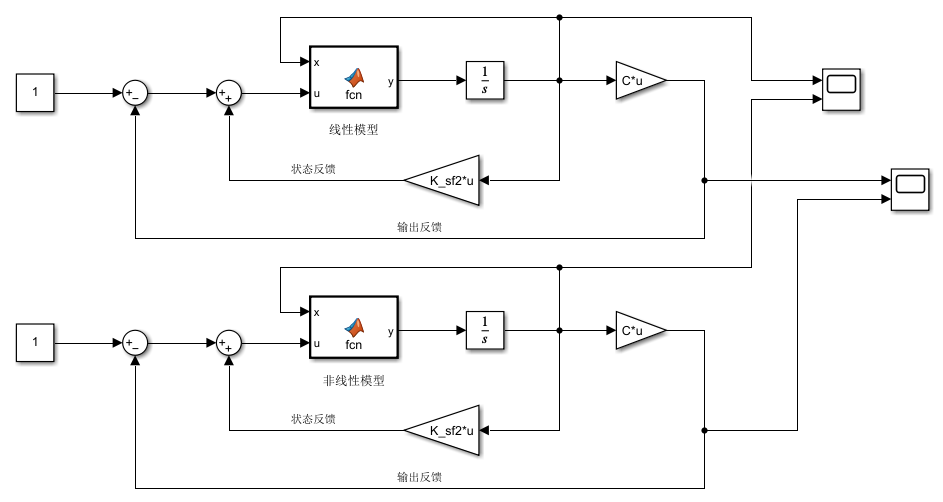
\includegraphics[width=.6\textwidth]{figure/倒立摆-输出反馈结构图.png} 
    \caption{基于原状态反馈的单位输出反馈控制器结构图} % caption是图片的标题
    % \label{img} % 此处的label相当于一个图片的专属标志,目的是方便上下文的引用
\end{figure}

在初始状态均为0的条件下,给定幅值为1的阶跃位移信号,其状态响应和输出响应曲线图如下所示:
\begin{figure}[H]
    \centering % 居中 
    % 图片文件的相对路径
    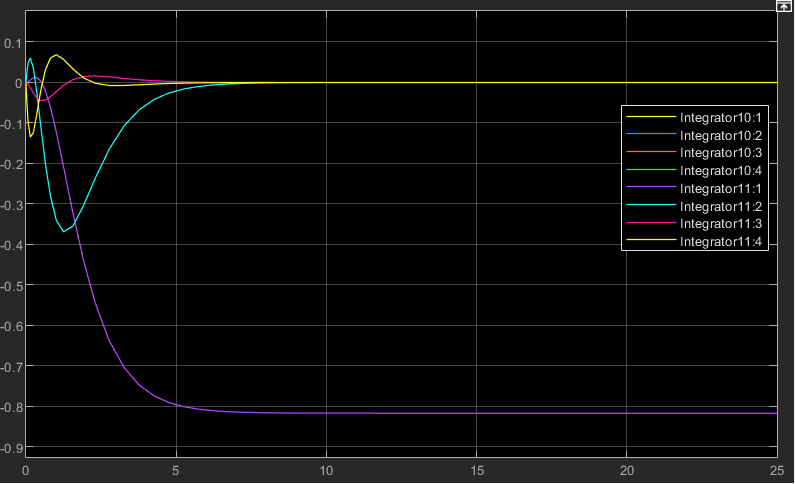
\includegraphics[width=.6\textwidth]{figure/倒立摆-输出反馈-响应对比.png} 
    \caption{输出反馈-状态响应对比图} % caption是图片的标题
    % \label{img} % 此处的label相当于一个图片的专属标志,目的是方便上下文的引用
\end{figure}
\begin{figure}[H]
    \centering % 居中 
    % 图片文件的相对路径
    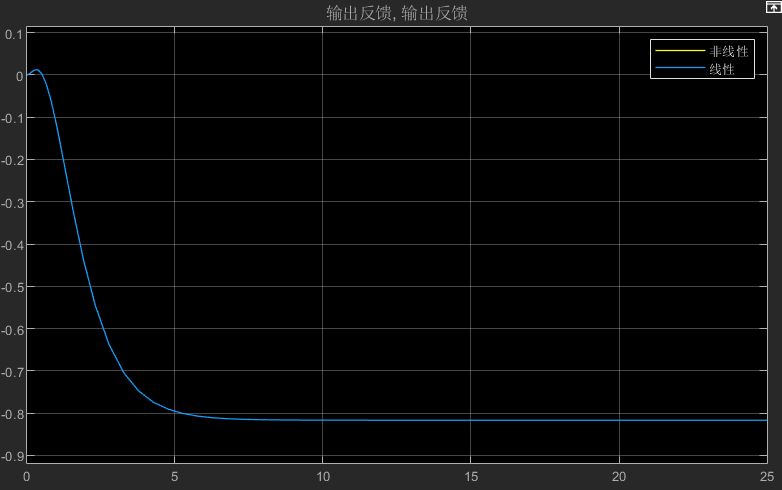
\includegraphics[width=.6\textwidth]{figure/倒立摆-输出反馈-输出对比.png}
    \caption{输出反馈-输出响应对比图} % caption是图片的标题
    % \label{img} % 此处的label相当于一个图片的专属标志,目的是方便上下文的引用
\end{figure}

由以上对比图容易看出,非线性模型和线性模型的状态响应曲线以及输出响应曲线几乎完全重合。这说明非线性和线性模型两者之间的差异已经小到可以忽略不计,同时也印证了对于非线性模型的简化处理是完全可行的。

%%%%
\paragraph{基于原状态反馈的带积分校正的输出反馈控制}~{}

% 1. 在原状态反馈结构基础上,引入带积分校正的输出反馈控制,实现跟踪位移信号
% 2. 基于线性模型,给定超调量和过渡时间要求,设计状态反馈控制器增益K1、积分增益K2
% 3. 基于simulink平台验证控制器效果:简化线性系统 + 控制策略
% 4. 基于simulink平台验证控制器效果:原始非线性系统 + 控制策略
% 5. 绘制两类闭环系统的输出响应曲线,比较异同与跟踪效果,分析原因

在原状态反馈结构基础上,引入带积分校正的输出反馈控制,其结构示意图如下所示:
\begin{figure}[H]
    \centering % 居中 
    % 图片文件的相对路径
    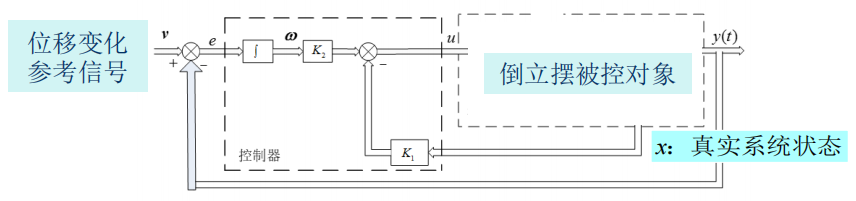
\includegraphics[width=.6\textwidth]{figure/倒立摆-带积分校正输出反馈.png}
    \caption{带积分校正的输出反馈示意图} % caption是图片的标题
    % \label{img} % 此处的label相当于一个图片的专属标志,目的是方便上下文的引用
\end{figure}

对于状态反馈控制器部分,其状态方程如下:
\begin{equation*}
	\begin{cases}
		\dot{x} = (A + BK_1)x + Bv_1 \\
		y = Cx
	\end{cases}
\end{equation*}

此外,根据输出反馈控制律,以及对于积分校正部分引入的一个新的状态分量$x_5$,有如下方程描述:
\begin{align*}
	v_1 &= K_2x_5 \\
	\dot{x}_5 &= v_2 - Cx
\end{align*}

对上述各方程组进行整理,即可得到在原状态反馈控制器基础上加入带积分补偿的输出反馈的系统的状态空间表达式:
\begin{equation*}
	\begin{cases}
		\dot{\overline{x}} = 
		\begin{bmatrix}
		\dot{x} \\
		\dot{x}_5
		\end{bmatrix} =
		\begin{bmatrix}
		A+BK_1 & BK_2 \\
		-C & 0
		\end{bmatrix}
		\begin{bmatrix}
		x \\
		x_5
		\end{bmatrix} +
		\begin{bmatrix}
		0 \\
		1
		\end{bmatrix}v \\
		
		y = Cx
	\end{cases}
\end{equation*}

接下来,需要基于上述线性系统模型,根据给定的超调量和过渡时间要求,计算得到状态反馈控制器增益$K_1$,以及积分增益$K_2$。根据经典的自动控制理论,可以得到基于二阶系统的超调量$\sigma$和阻尼比$\xi$之间的关系,其中通过阻尼比$\xi$计算超调量$\sigma$的公式如下所示:
\begin{equation*}
	\xi = \frac{\ln(1/\sigma)}{\sqrt{\pi^2 + (\ln(1/\sigma))^2}}
\end{equation*}

过渡时间又称为调节时间,用$t_s$表示。调节时间$t_s$与阻尼比$xi$、固有频率$\omega_n$之间存在如下关系:
\begin{equation*}
	t_s = 
	\begin{cases}
	\frac{3.5}{\xi\omega_n}, \quad \Delta = \pm5\% \\
	\\
	\frac{4.4}{\xi\omega_n}, \quad \Delta = \pm2\%
	\end{cases} \quad \quad 
	(0 < \xi < 0.8)
\end{equation*}

为便于理解上述公式,此处贴上其中涉及到的调节时间$t_s$、稳态误差$\Delta$等参数的示意图:
\begin{figure}[H]
    \centering % 居中 
    % 图片文件的相对路径
    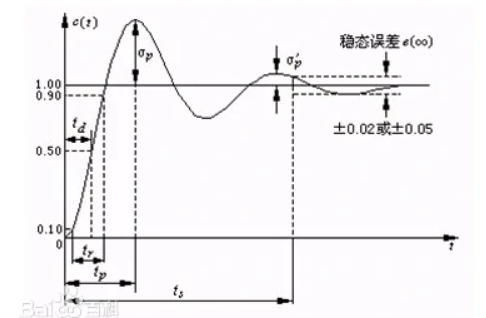
\includegraphics[width=.6\textwidth]{figure/调节时间示意图.png}
    \caption{调节时间与稳态误差示意图} % caption是图片的标题
    % \label{img} % 此处的label相当于一个图片的专属标志,目的是方便上下文的引用
\end{figure}

基于上述公式,我们就能通过给定的超调量和过渡时间要求,通过计算得到对应二阶系统的阻尼比$\xi$和固有频率$\omega_n$等参数,进而得到对应二阶系统的传递函数模型:
\begin{equation*}
	G(s) = \frac{\omega_n^2}{s^2 + 2\xi\omega_ns + \omega_n^2}
\end{equation*}

通过上述二阶系统的传递函数模型,将其转为零极点形式即可得到两个极点,我们将其作为本次设计的带积分校正的输出反馈-状态反馈控制系统的两个主导极点,以使得系统大致满足超调量和过渡时间的要求。事实上,本次设计的带积分校正的输出反馈-状态反馈控制器是一个5阶系统,因此除了两个主导极点之外,我们还需要配置其他3个非主导极点。为了尽可能避免这些非主导极点对系统性能的影响,需要满足在s平面让它们位于主导极点的左边,且远离主导极点。

这里我们指定超调量$\sigma$和调节时间$t_s$分别为:
\begin{equation*}
	\sigma = 0.2,\ t_s = 3
\end{equation*}

利用前述公式可以计算得到对应二阶系统的阻尼比$\xi$和固有频率$\omega_n$:
\begin{equation*}
	\xi = 0.4559,\ \omega_n = 3.2167
\end{equation*}

则对应二阶系统的传递函数模型及两个极点分别为:
\begin{equation*}
	G(s) = \frac{10.35}{s^2 + 2.933s + 10.35}
\end{equation*}
\begin{align*}
	p_1 &= -1.467 + 2.863i \\
	p_2 &= -1.467 - 2.863i
\end{align*}

加入其余的非主导极点后,最终的极点配置如下:
\begin{equation*}
	P_{inte} = [-1.467 + 2.863i,\ -1.467 - 2.863i,\ -6,\ -6,\ -6]
\end{equation*}

结合前述的系统状态空间模型,则可以得到系统的特征多项式以及期望的特征多项式:
\begin{equation*}
	f(\lambda) = |\lambda I - \begin{bmatrix}
		A+BK_1 & BK_2 \\
		-C & 0
	\end{bmatrix}|
\end{equation*}
\begin{equation*}
	f^*(\lambda) = \prod_{i = 1}^5 (\lambda - \lambda^*_i)
\end{equation*}

对比上述两特征多项式系数,令其分别相等即可求解得到状态反馈增益矩阵$K_1$以及积分增益$K_2$。此处使用MATLAB的$solve()$函数进行求解,其结果为:
\begin{align*}
	K_1 &= [89.342,\ 42.504,\ 141.025,\ 31.719] \\
	K_2 &= -114.032
\end{align*}

使用simulink分别搭建非线性和线性模型的带积分校正的输出反馈控制系统结构图如下:
\begin{figure}[H]
    \centering % 居中 
    % 图片文件的相对路径
    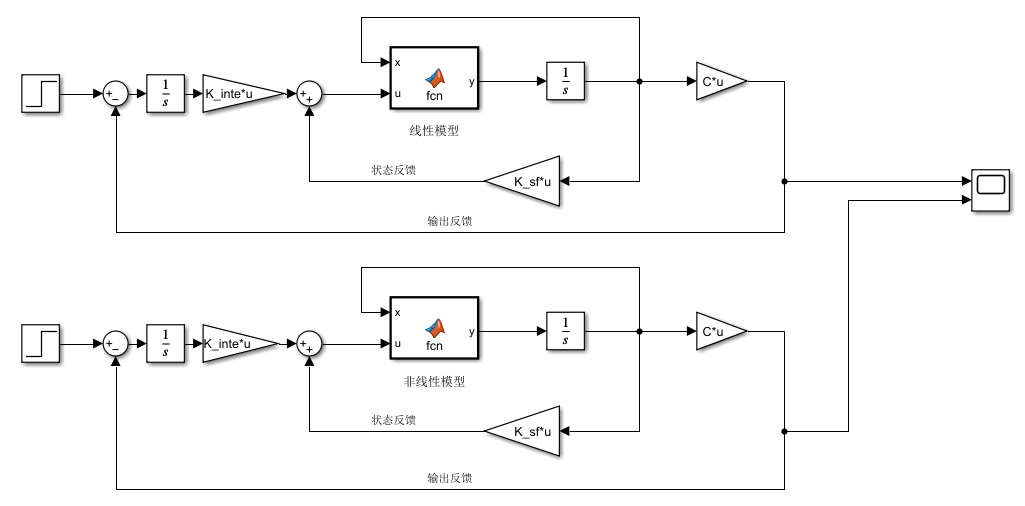
\includegraphics[width=.6\textwidth]{figure/倒立摆-积分校正-结构图.png}
    \caption{带积分校正的输出反馈系统结构图} % caption是图片的标题
    % \label{img} % 此处的label相当于一个图片的专属标志,目的是方便上下文的引用
\end{figure}

在初始状态均为零的条件下,在时间$t = 1$时刻给两个系统分别输入幅值为1的阶跃位移信号,其输出响应曲线如下所示:
\begin{figure}[H]
    \centering % 居中 
    % 图片文件的相对路径
    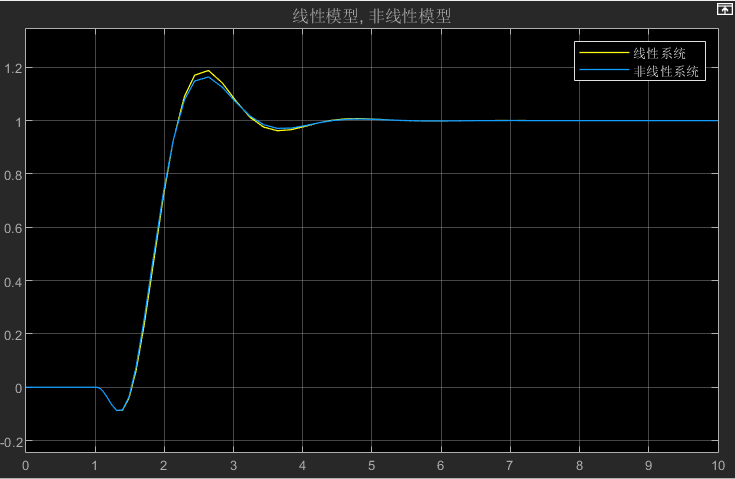
\includegraphics[width=.6\textwidth]{figure/倒立摆-积分校正-阶跃响应.png}
    \caption{带积分校正的输出反馈系统-阶跃响应} % caption是图片的标题
    % \label{img} % 此处的label相当于一个图片的专属标志,目的是方便上下文的引用
\end{figure}
可以看到,在阶跃信号作用下,系统能够迅速稳定在指定的位置;在调节过程中,系统的超调量大致为0.2,调节时间约为3s,其动态性能基本上满足我们的性能要求。可以注意到在上升阶段时两模型的响应曲线基本重合,在超调处没有完全重合,且非线性模型的超调量小于给定的指标,说明经过简化后的线性系统在某些方面仍在与真实系统存在差距。


%%%%
\paragraph{基于原状态反馈的带积分校正的输出反馈控制}~{}

% 1. 在基于状态观测器的状态反馈基础上,引入带积分校正的输出反馈控制,实现跟踪位移信号
% 2. 基于线性模型,给定超调量和过渡时间,设计状态反馈增益K1、积分增益K2、观测器增益G
% 3. 基于simulink平台验证控制效果:简化线性系统或原始非线性模型 + 控制策略
% 4. 绘制两类闭环系统的输出响应曲线,比较异同与跟踪效果,分析原因

在基于状态观测器的状态反馈基础上,引入带积分校正的输出反馈控制,其系统结构示意图如下:
\begin{figure}[H]
    \centering % 居中 
    % 图片文件的相对路径
    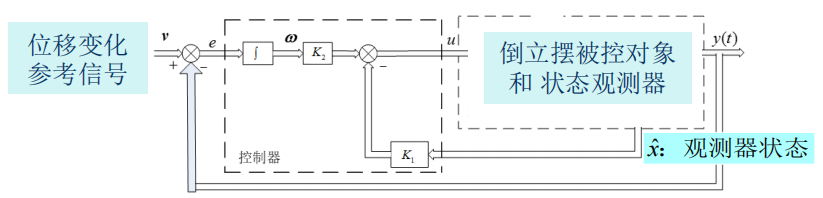
\includegraphics[width=.6\textwidth]{figure/倒立摆-积分校正-状态反馈-结构图示意.png}
    \caption{基于状态观测器状态反馈的带积分校正的输出反馈控制示意图} % caption是图片的标题
    % \label{img} % 此处的label相当于一个图片的专属标志,目的是方便上下文的引用
\end{figure}

给定超调量和过渡时间分别为$\sigma = 0.2,\ t_s = 3s$,选用前述基于状态反馈的带积分校正的输出反馈控制系统的状态反馈增益矩阵$K_1$及积分增益$K_2$,观测器极点设置为$p = [-1,\ -2,\ -3,\ -4]$,计算得到观测器增益矩阵为:
\begin{equation*}
	G = [10.00,\ 56.56,\ -271.02,\ -1268.81]^T
\end{equation*}

利用simulink分别搭建非线性模型与线性模型基于状态观测器状态反馈的带积分校正的输出反馈结构图,如下所示:
\begin{figure}[H]
    \centering % 居中 
    % 图片文件的相对路径
    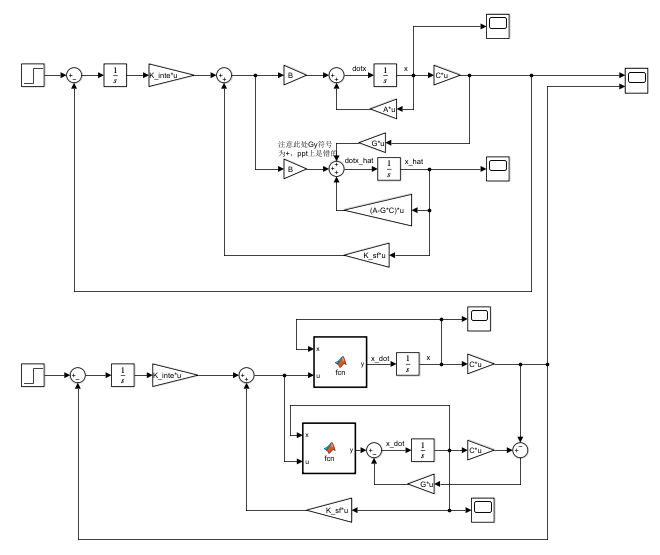
\includegraphics[width=.6\textwidth]{figure/倒立摆-积分校正-状态反馈-结构图.png}
    \caption{基于状态观测器状态反馈的带积分校正的输出反馈控制结构图} % caption是图片的标题
    % \label{img} % 此处的label相当于一个图片的专属标志,目的是方便上下文的引用
\end{figure}

在初始状态均为零的条件下,分别输入幅值为1的阶跃位移信号,在同一个示波器上观察两系统的响应曲线如下:
\begin{figure}[H]
    \centering % 居中 
    % 图片文件的相对路径
    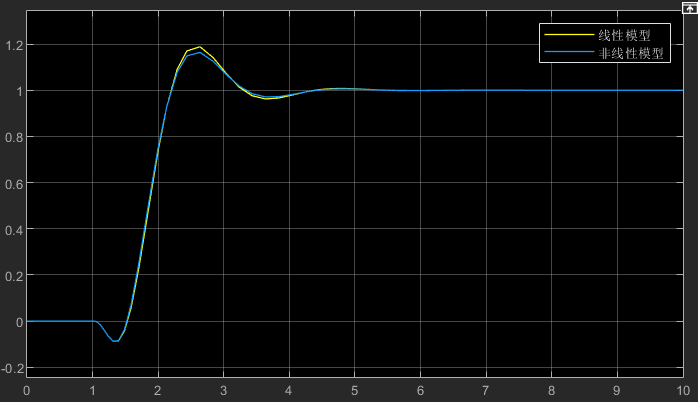
\includegraphics[width=.6\textwidth]{figure/倒立摆-积分校正-状态反馈-阶跃响应.png}
    \caption{基于状态观测器状态反馈的带积分校正的输出反馈控制系统阶跃响应} % caption是图片的标题
    % \label{img} % 此处的label相当于一个图片的专属标志,目的是方便上下文的引用
\end{figure}
可以看到,基于状态观测器状态反馈的带积分校正的输出反馈控制系统的阶跃响应与前述基于状态反馈的带积分校正的输出反馈控制系统基本一致,且不难看出其超调量和调节时间均满足上述要求。

%%%%
\paragraph{基于状态反馈的PID控制器}~{}

基于状态反馈,运用经典控制理论中的PID控制方法,引入PID控制器和输出反馈。利用simulink分别搭建非线性模型与线性模型的控制系统结构图,如下所示:
\begin{figure}[H]
    \centering % 居中 
    % 图片文件的相对路径
    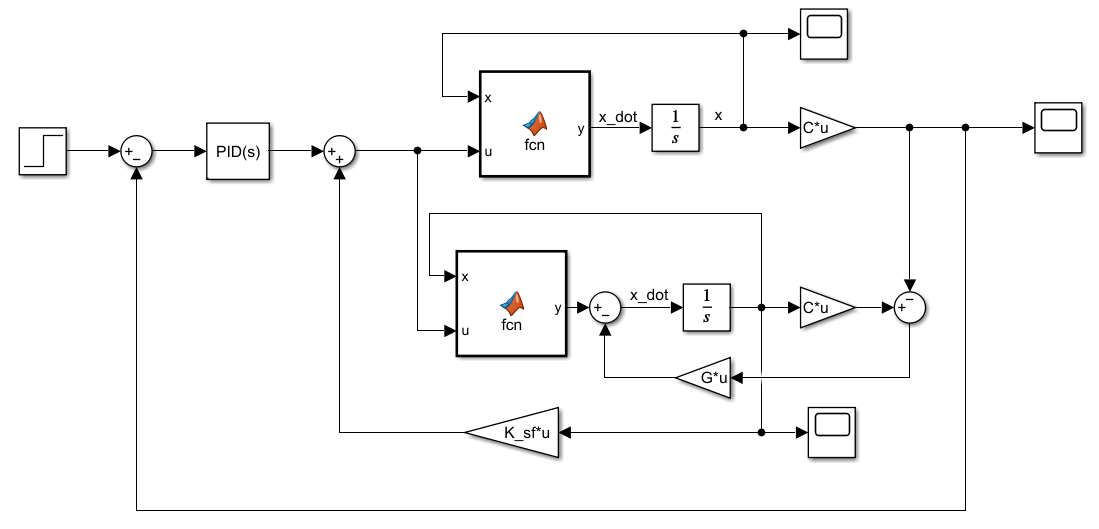
\includegraphics[width=.6\textwidth]{figure/倒立摆-非线性-pid-结构图.png}
    \caption{基于非线性系统状态反馈的PID控制系统} % caption是图片的标题
    % \label{img} % 此处的label相当于一个图片的专属标志,目的是方便上下文的引用
\end{figure}
\begin{figure}[H]
    \centering % 居中 
    % 图片文件的相对路径
    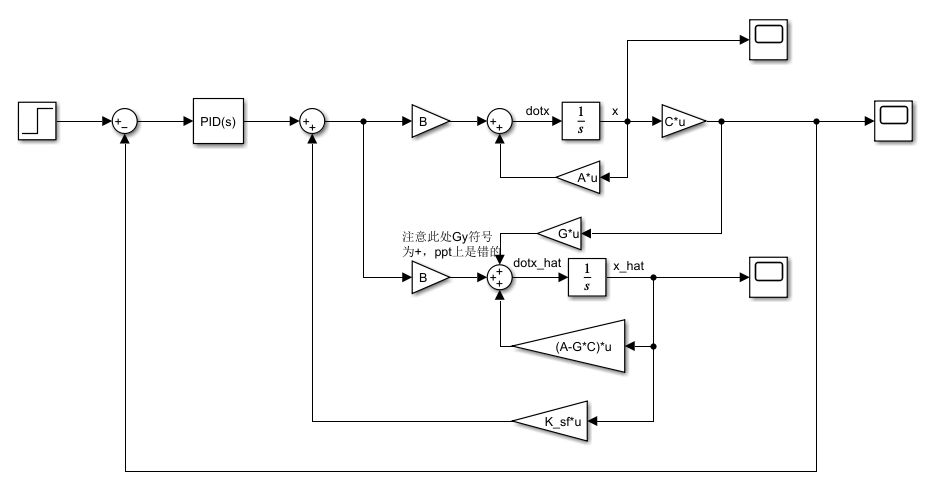
\includegraphics[width=.6\textwidth]{figure/倒立摆-线性-pid-结构图.png}
    \caption{基于线性系统状态反馈的PID控制系统} % caption是图片的标题
    % \label{img} % 此处的label相当于一个图片的专属标志,目的是方便上下文的引用
\end{figure}

使用MATLAB的PID调试工具,对两系统中的PID控制器进行调试。调试完毕后,在初始条件均为零的条件下,分别输入幅值为1的阶跃位移信号,观察系统输出,如下所示:
\begin{figure}[H]
    \centering % 居中 
    % 图片文件的相对路径
    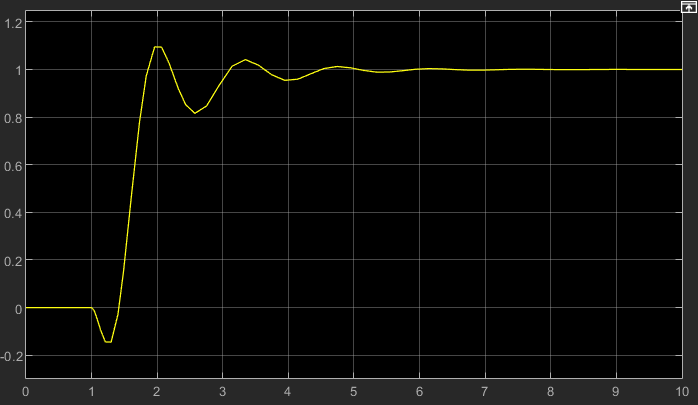
\includegraphics[width=.6\textwidth]{figure/倒立摆-非线性-pid-输出.png}
    \caption{基于非线性系统状态反馈的PID控制系统阶跃响应} % caption是图片的标题
    % \label{img} % 此处的label相当于一个图片的专属标志,目的是方便上下文的引用
\end{figure}
\begin{figure}[H]
    \centering % 居中 
    % 图片文件的相对路径
    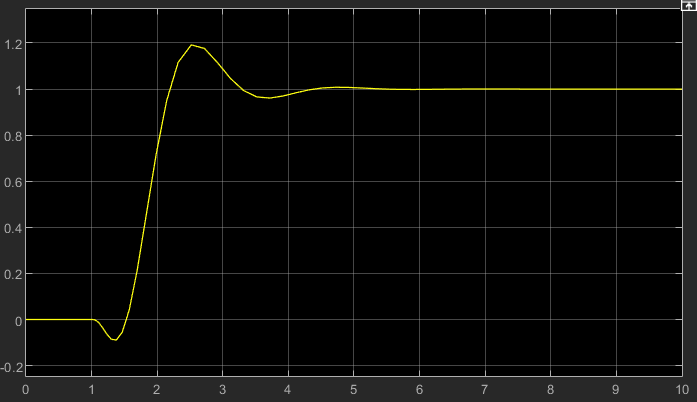
\includegraphics[width=.6\textwidth]{figure/倒立摆-线性-pid-输出.png}
    \caption{基于线性系统状态反馈的PID控制系统阶跃响应} % caption是图片的标题
    % \label{img} % 此处的label相当于一个图片的专属标志,目的是方便上下文的引用
\end{figure}
可以看到,线性模型在PID控制器作用下基本可以达到所要求的性能指标,其超调量约为0.2,调节时间约为3s;而非线性模型由于其非线性特性,在PID控制器作用下达到的性能表现会稍弱于线性模型。

%
\section{设计二:蔡氏混沌电路}
%%
\subsection{任务概述}
%%%
\paragraph{系统模型建立}~{}
\begin{itemize}
	\item 基于电学知识建立机理非线性模型;
	\item 基于simulink搭建结构模型。
\end{itemize}

%%%
\paragraph{混沌现象分析}~{}
\begin{itemize}
	\item 分析系统响应,绘制并比较响应曲线和状态轨迹;
	\item 分析并获取混沌信号。
\end{itemize}

%%%
\paragraph{同构主从系统同步设计与验证}~{}
\begin{itemize}
	\item 搭建结构相同的主从两个系统,从系统需要加输出反馈控制;
	\item 基于李雅普诺夫理论,得到控制器设计条件;
	\item 设计输出反馈控制器;
	\item 基于simulink验证控制效果。
\end{itemize}

%%%
\paragraph{保密通信应用}~{}
\begin{itemize}
	\item 基于混沌信号,实现主系统的信号加密;
	\item 利用被控从系统实现同步信号解密。
\end{itemize}

%%
\subsection{模型与分析}
%%%
\subsubsection{系统模型建立}
蔡氏混沌电路的电路结构图如下左图所示,其中包含一个非线性电阻元件,其伏安特性曲线如下右图所示:
\begin{figure}[htbp]
	\centering
	\begin{minipage}{0.49\linewidth}
		\centering
		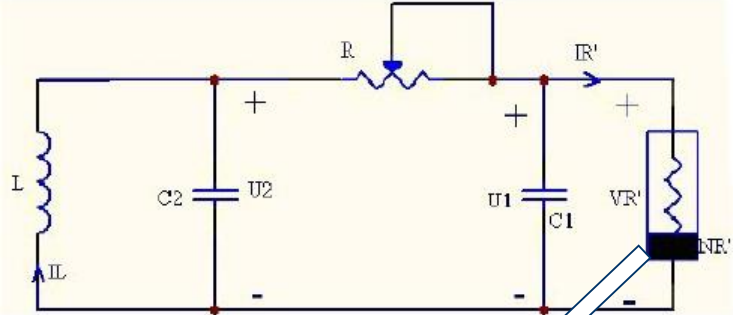
\includegraphics[width=1\linewidth]{figure/混沌电路结构.png}
		\caption{蔡氏混沌电路结构}
		\label{label1} %文中引用该图片代号
	\end{minipage}
	%\qquad
	\begin{minipage}{0.49\linewidth}
		\centering
		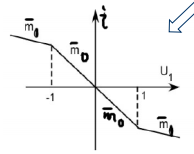
\includegraphics[width=0.6\linewidth]{figure/非线性元件伏安特性曲线.png}
		\caption{非线性元件的伏安特性}
		\label{label2} %文中引用该图片代号
	\end{minipage}
\end{figure}

根据基尔霍夫电流定律和电压定律,可以用如下方程组来描述该电路:
\begin{equation*}
	\begin{cases}
		C_1\frac{dU_1}{dt} = 
		\frac{U_2 - U_1}{R} - h(U_1) \\
		C_2\frac{dU_2}{dt} = \frac{U_1 - U_2}{R} + i_L \\
		L\frac{di_L}{dt} = -U_2
	\end{cases}
\end{equation*}

同时,根据非线性电阻元件的伏安特性曲线,可以用分段函数对其特性进行描述:
\begin{equation*}
	g(U_1) = 
	\begin{cases}
		\overline{m}_1U_1 + \overline{m}_0 - \overline{m}_1, \quad U_1 > 1 \\
		\overline{m}_0U_1, \quad |U_1| \le 1 \\
		\overline{m}_1U_1 - \overline{m}_0 + \overline{m}_1, \quad U_1 < -1
	\end{cases}
\end{equation*}

可以进一步整理为:
\begin{equation*}
	g(U_1) = \overline{m}_1U_1 + \frac{\overline{m}_0 - \overline{m}_1}{2}(|U_1 + 1| - |U_1 - 1|)
\end{equation*}

对上述各式中的变量做如下定义:
\begin{equation*}
	\begin{cases}
		x_1 = U_1 \\
		x_2 = U_2 \\
		x_3 = Ri_L \\
		y = x_1 \\
		t = RC_2\tau \\
		a = \frac{C_2}{C_1} \\
		b = \frac{R^2C_2}{L} \\
		m_0 = R\overline{m}_0 + 1 \\
		m_1 = R\overline{m}_1 + 1 \\
		h(x_1) = Rg(x_1) + x_1
	\end{cases}
\end{equation*}

其中参数的取值为:
\begin{equation*}
	\begin{cases}
		a = 9 \\
		b = 14.28 \\
		m_0 = -1/7 \\
		m_1 = 2/7
	\end{cases}
\end{equation*}

将上述定义代入方程组,即可解得状态空间表达式:
\begin{equation*}
	\begin{bmatrix}
		\dot{x}_1 \\
		\dot{x}_2 \\
		\dot{x}_3 \\
	\end{bmatrix} = 
	\begin{bmatrix}
		-am_1 & a & 0 \\
		1 & -1 & 1 \\
		0 & -b & 0
	\end{bmatrix}
	\begin{bmatrix}
		x_1 \\
		x_2 \\
		x_3 \\
	\end{bmatrix} + 
	\begin{bmatrix}
		-a(m_0 - m_1) \\
		0 \\
		0 \\
	\end{bmatrix} \cdot \frac{|x_1 + 1| - |x_1 - 1|}{2}
\end{equation*}

可最终整理为如下形式:
\begin{equation*}
	\begin{cases}
		\dot{x} = Ax + H\sigma(Dx) \\
		y = Cx
	\end{cases}
\end{equation*}

其中:
\begin{equation*}
	\sigma(Dx) = \frac{|x_1 + 1| - |x_1 - 1|}{2},  
	A = \begin{bmatrix}
		-am_1 & a & 0 \\
		1 & -1 & 1 \\
		0 & -b & 0
	\end{bmatrix},  
	H = \begin{bmatrix}
		-a(m_0 - m_1) \\
		0 \\
		0 \\
	\end{bmatrix},  
	C = [1 \quad 0 \quad 0]
\end{equation*}

%%%
\subsubsection{系统响应分析}
使用simulink搭建混沌电路模型,如下所示:
\begin{figure}[H]
    \centering % 居中 
    % 图片文件的相对路径
    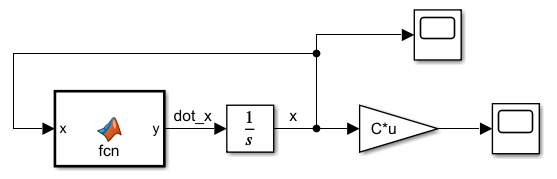
\includegraphics[width=.6\textwidth]{figure/混沌电路-系统结构图.png}
    \caption{混沌电路系统结构图} % caption是图片的标题
    % \label{img} % 此处的label相当于一个图片的专属标志,目的是方便上下文的引用
\end{figure}
在初始值分别为$[0.01,\ 0,\ 0]$的条件下,混沌电路的输出如下图所示:
\begin{figure}[H]
    \centering % 居中 
    % 图片文件的相对路径
    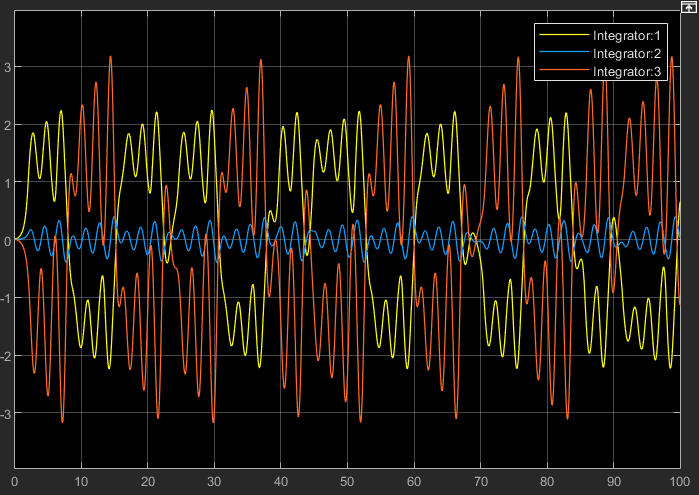
\includegraphics[width=.6\textwidth]{figure/混沌电路-单个系统输出.png}
    \caption{混沌电路输出$[0.01,\ 0,\ 0]$} % caption是图片的标题
    % \label{img} % 此处的label相当于一个图片的专属标志,目的是方便上下文的引用
\end{figure}
改变初始值为$[1,\ 0,\ 0]$的条件下,混沌电路的输出如下图所示:
\begin{figure}[H]
    \centering % 居中 
    % 图片文件的相对路径
    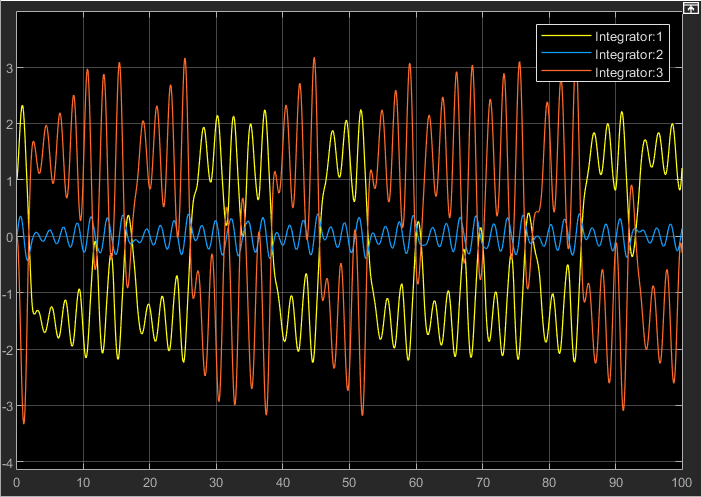
\includegraphics[width=.6\textwidth]{figure/混沌电路-单个系统输出2.png}
    \caption{混沌电路输出$[1,\ 0,\ 0]$} % caption是图片的标题
    % \label{img} % 此处的label相当于一个图片的专属标志,目的是方便上下文的引用
\end{figure}
蔡氏混沌电路是一种对于初始状态十分敏感的系统,由上面的结果可以看出,在不同的初始状态下,系统的输出信号是完全不同的。

对于混沌电路的输出,还可以通过相图的形式更加直观地展示:
\begin{figure}[H]
    \centering % 居中 
    % 图片文件的相对路径
    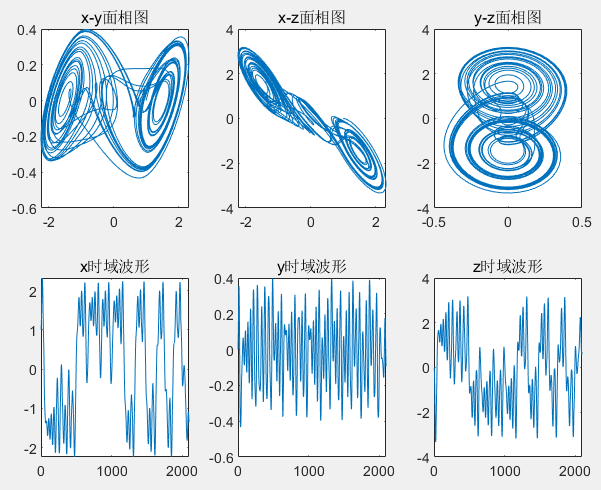
\includegraphics[width=.6\textwidth]{figure/混沌电路-输出.png}
    \caption{混沌电路相图} % caption是图片的标题
    % \label{img} % 此处的label相当于一个图片的专属标志,目的是方便上下文的引用
\end{figure}

%%
\subsection{同步设计与验证}
% 1. 具有相同结构的 主系统M 和 从系统S(初态不
% 同),通过设计控制器C,使得从系统状态跟踪主
% 系统状态
% 2. 利用李亚普洛夫稳定性理论,建立控制器增益K应
% 满足的条件(已给出,报告应含关键过程)
% 3. 利用LMI工具箱,求出控制器增益
% 4. 利用simulink,验证同步控制效果
% 5. 尝试其他类型控制(PID,模糊控制,等),选做

通过设计具有相同结构的主系统M和从系统S,以及一个控制器C,使得从系统的状态可以跟踪主系统的状态。

%%%
\subsubsection{同步控制设计条件分析}
%%%%
\paragraph{系统方程及同步误差系统建立}~{}

主系统M、从系统S和控制器C的表达式描述如下:
\begin{align*}
	M&:\begin{cases}
		\dot{x} = Ax(t) + H\sigma(Dx(t)) \\
		p(t) = Cx(t)
	\end{cases} \\
	S&:\begin{cases}
		\dot{z} = Az(t) + H\sigma(Dz(t)) + u(t) \\
		q(t) = Cz(t)
	\end{cases} \\
	C&: u(t) = K(p(t) - q(t))
\end{align*}

定义同步误差为:
\begin{align*}
	e(t) &= x(t) - z(t) \\
	y(De) &= \sigma(Dx) - \sigma(Dz)
\end{align*}

则可以得到一个同步误差系统,其状态方程可表示为:
\begin{equation*}
	\dot{e} = (A - KC)e + Hy(De)
\end{equation*}

%%%%
\paragraph{非线性函数的约束条件推导}~{}

对于非线性函数:
\begin{equation*}
	\sigma(Dx) = \frac{|x_1 + 1| - |x_1 - 1|}{2}
\end{equation*}

根据其对应曲线的斜率特性,可以知道:
\begin{equation*}
	0 \le \frac{\sigma(s_1) - \sigma(s_2)}{s_1 - s_2} \le 1
\end{equation*}

继而可以得到:
\begin{equation*}
	\frac{y(Dz)}{De} = \frac{\sigma(Dx) - \sigma(Dz)}{Dx - Dz} \in [0,\ 1]
\end{equation*}

因此,当$T = T^T > 0$时,有:
\begin{equation*}
	y^T(Dz)T[De - y(Dz)] + [De - y(Dz)]^T Ty(Dz) > 0
\end{equation*}
即:
\begin{equation*}
	\begin{bmatrix}
		e \\
		y(Dz) 
	\end{bmatrix}^T 
	\begin{bmatrix}
		0 & D^T T \\
		TD & -2T
	\end{bmatrix}
	\begin{bmatrix}
		e \\
		y(Dz)
	\end{bmatrix} > 0
\end{equation*}

%%%%
\paragraph{同步控制设计条件推导}~{}

定义函数:
\begin{equation*}
	V(e) = e^T(t)Pe(t),\ P = P^T > 0
\end{equation*}

求导可以得到:
\begin{align*}
	\dot{V}(e(t)) &= 2e^T(t)P[(A - KC)e(t) + Hy(Dz(t))] \\
	&= \begin{bmatrix}
		e(t) \\
		y(Dz(t))
	\end{bmatrix}^T 
	\begin{bmatrix}
		P(A - KC) + (A - KC)^TP^T & PH \\
		H^TP^T & 0
	\end{bmatrix}
	\begin{bmatrix}
		e(t) \\
		y(Dz(t))
	\end{bmatrix} \quad (A)
\end{align*} 

结合上述得到的非线性函数约束:
\begin{equation*}
	\begin{bmatrix}
		e \\
		y(Dz) 
	\end{bmatrix}^T 
	\begin{bmatrix}
		0 & D^T T \\
		TD & -2T
	\end{bmatrix}
	\begin{bmatrix}
		e \\
		y(Dz)
	\end{bmatrix} > 0 \quad (B)
\end{equation*}

则有:
\begin{align*}
	\dot{V}(e(t)) &= (A) \le (A) + (B) \\
	&= \begin{bmatrix}
		e(t) \\
		y(Dz(t))
	\end{bmatrix}^T 
	\begin{bmatrix}
		PA - PKC + A^TP - C^TK^TP & PH + D^TW^TT \\
		T^TWD + H^TP^T & -2T
	\end{bmatrix}
	\begin{bmatrix}
		e(t) \\
		y(Dz(t))
	\end{bmatrix}
\end{align*}

为方便表述,此处令:
\begin{equation*}
	\begin{bmatrix}
		PA - PKC + A^TP - C^TK^TP & PH + D^TW^TT \\
		T^TWD + H^TP^T & -2T
	\end{bmatrix} = (C)
\end{equation*}

由于$V = PK$,则$K = P^{-1}V$,代入(C)中可以得到:
\begin{equation*}
	(C) = \begin{bmatrix}
		PA - VC + A^TP - C^TV^T & PH + D^TW^TT \\
		T^TWD + H^TP^T & -2T
	\end{bmatrix}
\end{equation*}

其中$W = I$。此时若$P > 0$,则有$V(e(t)) > 0,\ (C) < 0$,则$\dot{V}(e(t)) < 0$,由稳定性判据可知此时系统是渐进稳定的。

根据上述推导,可以使用LMI方法基于以下条件进行求解:
\begin{equation*}
	P > 0,\ T > 0,\ 
	\begin{bmatrix}
		PA - VC + A^TP^T - C^TV^T & PH + D^TT \\
		T^TD + H^TP^T & -2T	
	\end{bmatrix} < 0
\end{equation*}

同时,增益矩阵$K$可由以下公式得到:
\begin{equation*}
	K = P^{-1}V
\end{equation*}

%%%
\subsection{同步效果仿真验证}
利用simulink搭建同构主从蔡氏混沌电路系统,其总体结构图和各部分结构图如下所示:
\begin{figure}[htbp]
	\centering
	\begin{minipage}{0.49\linewidth}
		\centering
		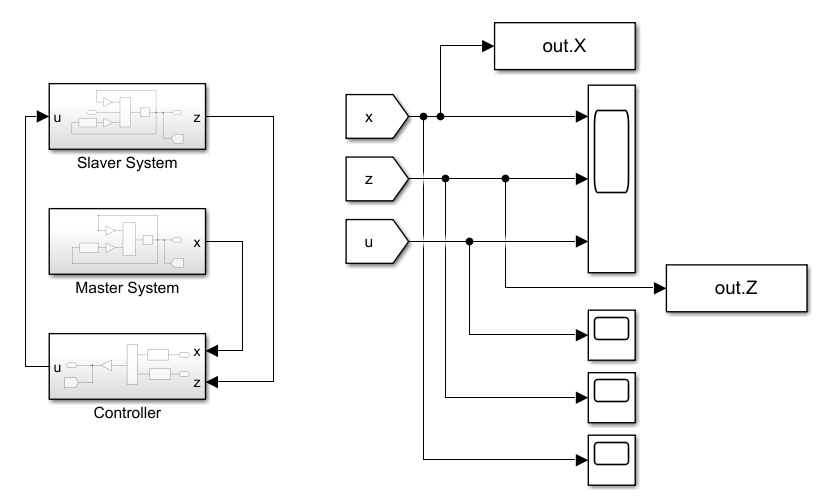
\includegraphics[width=0.9\linewidth]{figure/混沌电路-总体.png}
		\caption{同步主从混沌电路系统总体结构}
		% \label{label1} %文中引用该图片代号
	\end{minipage}
	%\qquad
	\begin{minipage}{0.49\linewidth}
		\centering
		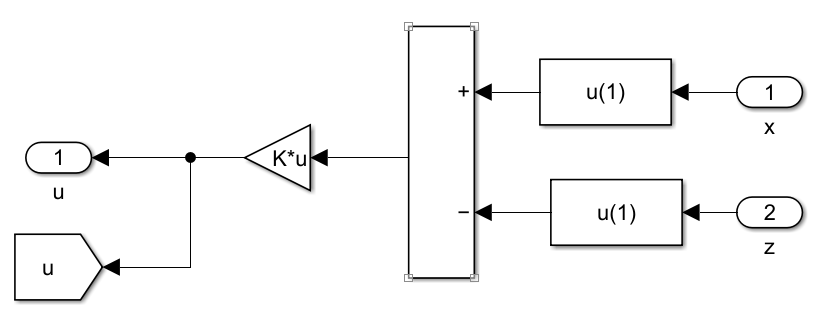
\includegraphics[width=0.9\linewidth]{figure/混沌电路-controler.png}
		\caption{控制器结构图}
		% \label{label2} %文中引用该图片代号
	\end{minipage}
\end{figure}
\begin{figure}[htbp]
	\centering
	\begin{minipage}{0.49\linewidth}
		\centering
		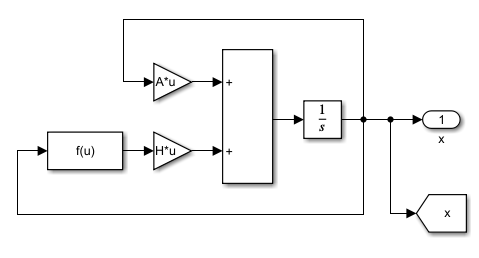
\includegraphics[width=0.9\linewidth]{figure/混沌电路-master.png}
		\caption{主系统结构图}
		% \label{label1} %文中引用该图片代号
	\end{minipage}
	%\qquad
	\begin{minipage}{0.49\linewidth}
		\centering
		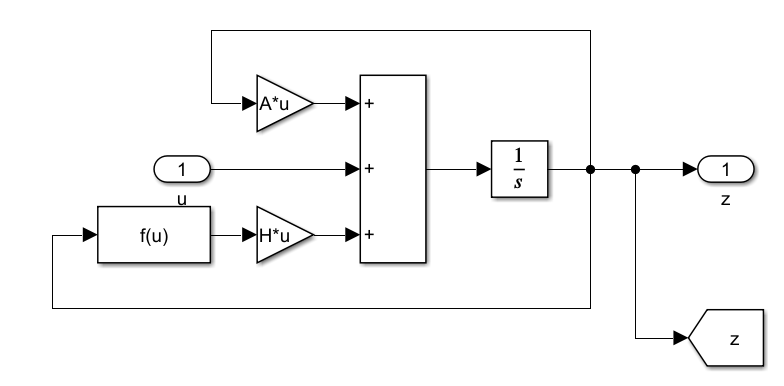
\includegraphics[width=0.9\linewidth]{figure/混沌电路-slaver.png}
		\caption{从系统结构图}
		% \label{label2} %文中引用该图片代号
	\end{minipage}
\end{figure}

基于前述的同步控制条件,使用LMI方法对控制器增益$K$进行求解,其结果为:
\begin{equation*}
	K = [1.146,\ 1.708,\ -0.013]^T
\end{equation*}

将主、从系统输出信号放在同一个示波器上进行对比显示,如下所示:
\begin{figure}[H]
    \centering % 居中 
    % 图片文件的相对路径
    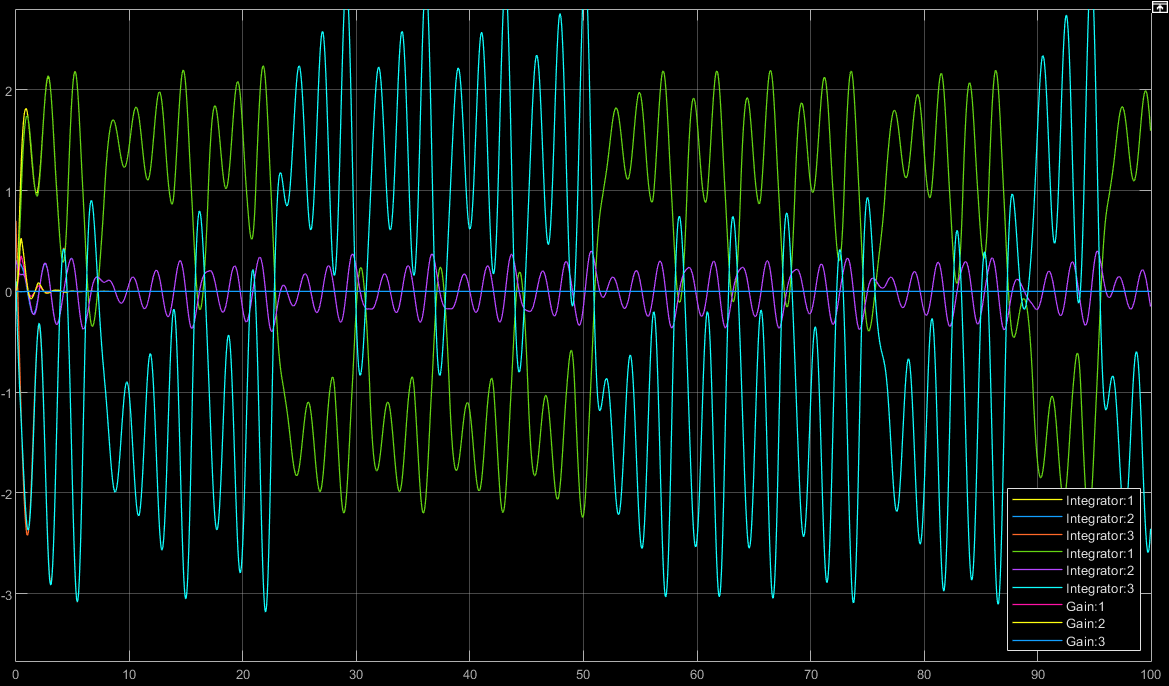
\includegraphics[width=.6\textwidth]{figure/混沌电路-同步-输出.png}
    \caption{同步主从混沌电路系统输出对比} % caption是图片的标题
    % \label{img} % 此处的label相当于一个图片的专属标志,目的是方便上下文的引用
\end{figure}
容易看出,主、从系统的各状态输出信号基本重合,说明控制器增益$K$的设计是合理的,且控制器的效果较为理想。

%%
\subsection{保密通信应用}
% 发送端:把混沌信号(主系统产生)加入待发信号中,加密
% 网络中:传输的混合信号(待发信号+混沌信号)
% 接收端:把收到混合信号去掉混沌信号(从系统产生),解密
% 需要控制从系统信号与主系统信号同步

在发送端,利用混沌电路产生的混沌信号,采用某种算法对图像进行加密处理后发送;在接收端接收到混合信号后,使用基于从系统产生的混沌信号,以相应的算法对混合信号进行解密,最终得到原来的图像数据。

将产生的3路混沌信号进行归一化处理,并且按RGB格式将其范围限制在$[0,\ 255]$区域内。对于待发送的图像,将其按RGB通道信号进行分离,并将每个通道的数据与混沌信号进行按位或的操作(加密),即可得到加密后的图像。在对图像进行解密时,只需使用来自从系统的相同的混沌信号,对加密图像的各通道数据再做一次按位或的操作即可得到原图像。运行结果如下图所示:
\begin{figure}[htbp]
	\centering
	\begin{minipage}{0.49\linewidth}
		\centering
		
\includegraphics[width=0.9\linewidth]{figure/混沌电路-原图像.png}
		\caption{原图像}
		% \label{label1} %文中引用该图片代号
	\end{minipage}
	%\qquad
	\begin{minipage}{0.49\linewidth}
		\centering
		
\includegraphics[width=0.9\linewidth]{figure/混沌电路-解密图像.png}
		\caption{解密图像}
		% \label{label2} %文中引用该图片代号
	\end{minipage}
\end{figure}

该过程中产生的加密图像如下图所示:
\begin{figure}[H]
    \centering % 居中 
    % 图片文件的相对路径
    \includegraphics[width=.6\textwidth]{figure/混沌电路-加密图像.png}
    \caption{加密图像} % caption是图片的标题
    % \label{img} % 此处的label相当于一个图片的专属标志,目的是方便上下文的引用
\end{figure}

%
\section{心得与体会}

\paragraph{倒立摆}~{}

在设计基于原状态反馈的单位输出反馈控制系统,以及带积分校正的输出反馈控制系统时,要求控制系统需要满足给定的超调量和过渡时间性能指标,并以此来确定控制系统的参数。这个问题不同于前面比较常规的设计要求,我最初没有什么思路。

通过查阅一些资料发现,要使得控制系统满足某种性能指标,有这样一种解决方法:把高阶系统近似当做一个典型二阶系统进行处理,这样对系统的分析就会更加容易。结合在经典控制理论中学到的相关知识,基于典型的二阶系统,可以得到系统超调量、过渡时间等性能指标与系统阻尼比和自然频率等系统参数之间的转换关系,并由此得到给定的性能指标对应的二阶系统的传递函数。

然后,为了进一步得到高阶系统的参数,利用我们得到的二阶系统的传递函数,将它的极点作为高阶系统的主导极点,以使得高阶系统的性能可以与该二阶系统在一定程度上保持一致。

对于高阶系统,把除主导极点以外的其他极点按照一般要求配置好以后,就可以根据给定的极点通过计算得到高阶系统的参数。此外还要注意一点,需要把高阶系统先用状态空间模型描述出来,之后我们得到的系统参数也是该模型中的参数。

本次控制理论课程设计中,对于倒立摆控制系统设计的训练,进一步加深了我对控制系统理论的理解,而且更重要的是使我掌握了一些控制系统设计的一般步骤和常用处理方法,这些知识在实际的应用中显然是更为重要的。

\paragraph{蔡氏混沌电路}~{}

蔡氏混沌电路是一种复杂的非线性系统,而且对于系统初始状态等系统参数是十分敏感的,任何微小的差异都有可能导致系统呈现出截然不同的状态。蔡氏混沌电路的这种特点也使得它在信号加密等研究领域备受欢迎。本次课程设计中我们同样使用了蔡氏混沌电路来实现图像传输过程中的简单加密和解密功能,在学习控制系统设计的同时也拓宽了我们的知识面。最后非常感谢老师的教学,在这个过程中我学到了很多新的知识和实用的技能,希望以后可以将它们应用于解决实际的问题。



\newpage
%
\section{附录}
%
\paragraph{附录一:倒立摆程序}
\begin{lstlisting}
clc, clear

%% 倒立摆参数
m = 0.1;
M = 1;
l = 0.5;
g = 9.8;

%% 机理非线性模型
% x1_dot = x2;
% x2_dot = (u+m*l*x4^2*sin(x3)-m*g*sin(x3)*cos(x3))/(M+m-m*cos(x3)^2);
% x3_dot = x4;
% x4_dot = (-u*cos(x3)+(M+m)*g*sin(x3)-m*l*x4^2*sin(x3)*cos(x3))/((M+m)*l-m*l*cos(x3)^2);

%% 简化后的线性模型
% x1_dot = x2;
% x2_dot = (u-m*g*x3) / M;
% x3_dot = x4;
% x4_dot = (-u + (M+m)*g*x3) / (M*l);
A = [0 1 0 0; 0 0 -m*g/M 0; 0 0 0 1; 0 0 (M+m)*g / (M*l) 0];
B = [0; 1/M; 0; -1/(M*l)];
C = [1 0 0 0];
D = 0;
sys_ss = ss(A, B, C, D);

%% 传递函数模型  
[z,p,xi] = ss2zp(A,B,C,D);
[num,den] = zp2tf(z,p,xi);
sys_tf1 = zpk(z,p,xi);
sys_tf2 = tf(num,den);

% 阶跃响应
figure, step(sys_tf1)
% figure, step(sys_tf2)

% 传递函数分解 用于搭建结构模型
b = [1 0  -19.6];
a = [1 0 -21.56 0 0];
[r, p, xi] = residue(b, a);
% sys1 = tf([r(1)], [1 -p(1)])
% sys2 = tf([r(2)], [1 -p(2)])
% sys3 = tf([r(3)], [1 -p(3)])
% sys4 = tf([r(4)], [1 -p(4)])
% sys = sys1 + sys2 + sys3 + sys4

%% 传递函数模型 稳定性分析 nyquist图
figure(1);
nyquist(sys_tf1);
% nyquist(sys_tf2);

%% 传递函数模型 系统性能分析 bode图
figure(2);
% Bode响应 指示幅值和相位裕度
margin(sys_tf1);
grid on;
% 获取裕度值(不绘图)
[Gm, Pm, Wcg, Wcp] = margin(sys_tf1)
magdb = 20*log10(Gm);

%% 基于状态空间表达式稳定性判断
%LMI方法(间接法) 李二判别法
P_SF = sdpvar(4, 4, 'symmetric');
Fcond = [P_SF>=0, A'*P_SF+P_SF*A<=0];%注意严格大于等于
ops = sdpsettings('verbose', 0, 'solver', 'sedumi');%设置求解环境
diagnostics = solvesdp(Fcond, [], ops);%迭代求解
[m, p] = checkset(Fcond);%返回求解结果
tmin = min(m);%验证是否满足
if tmin > 0
    disp('稳定')
else 
    disp('不稳定')
end

%李一 直接法
lambda = eig(A);
% all: 任意都满足 real: 取实部
reflag = all(real(lambda) < 0);
if reflag
    disp('稳定')
else
    disp('不稳定')
end

%% 李二 思路二判断稳定性 方程无解或多解 可能不能使用该方法
% Q = eye(size(A, 1));
% % 求李雅普诺夫方程
% P = lyap(A, Q);
% % 利用希尔维斯特判据判断P的正定性
% det1 = det(P(1, 1));
% det2 = det(P(1 : 2, 1 : 2));
% det3 = det(P(1 : 3, 1 : 3));
% det4 = det(P);
% Det = [det1; det2; det3; det4];
% if min(Det) > 0
%     '系统稳定'
% else
%     '系统不稳定'
% end

%% 状态空间模型 能控能观性分析
%秩判据
n = size(A, 1);
Qc = ctrb(A, B);
Qo = obsv(A, C);
if rank(Qc) == n
    disp('系统能控,可通过状态反馈任意配置极点')
else
    disp('系统不完全能控')
end
if rank(Qo) == n
    disp('系统能观,可任意配置观测器系统极点')
else
    disp('系统不完全能观')
end

%约旦标准型
[T, J] = jordan(A);
A_jordan = T' * A * T
B_jordan = T' * B
C_jordan =  C * T
%能控:约旦块对应的B末尾行非全零
%能观:约旦块对应的C首列非全零

%% 状态反馈SF 给定极点配置 获取状态反馈增益K
P_sf = [-1, -2, -3, -4];
% 计算给定极点下的状态反馈增益
% 注意这里的状态反馈增益的符号与书上相反
K_sf = -acker(A, B, P_sf);

%%  输出反馈的反馈增益固定为1 只需使用上面的状态反馈增益K_sf-C
K_sf2 = K_sf + C

%% 基于状态观测器的状态反馈OSF 给定观测器极点配置 获取反馈矩阵G
P_osf = [-1, -2, -3, -4];
% 计算给定极点下的状态观测器输出误差反馈矩阵
G = (acker(A', C', P_osf))';

%%%%%%%%%%%%%%%%%%%%%%%%%%%%%%%%%%%%%%%%%%%%%
%% 带积分补偿的输出反馈-状态反馈控制器
% 给定超调量和调节时间 计算阻尼比和频率
% 此处将原系统近似为二阶系统处理 得到的两个极点作为主导极点 
sigma = 0.2; % 超调量
ts = 3; % 调节时间
% 计算阻尼比 log()-自然对数
pi = 3.14159;
xi = log(1/sigma) / sqrt(pi^2 + log(1/sigma)^2);
% 计算固有频率 Delta = 5%
wn = 4.4 / (xi * ts);
[z, p, k] = tf2zp([wn^2], [1, 2*xi*wn, wn^2]);
tf([wn^2], [1, 2*xi*wn, wn^2])
% p % 得到主导极点
% 添加的其他极点要向左远离主导极点 减小对上面超调量 调节时间指标的影响
P_inte = [p(1), p(2), -6, -6, -6];

%% 带积分校正的输出反馈
syms k1 k2 k3 k4 k5 s
K = [k1 k2 k3 k4 k5];
A_new = [A+B*K(1:4), B*K(5); -C, 0];
an = charpoly(A_new); % 系统特征多项式系数
an_star = poly(P_inte); % 期望特征多项式系数
% 求解增益
K = solve(an(1) == an_star(1), ...
                an(2) == an_star(2), ...
                an(3) == an_star(3), ...
                an(4) == an_star(4), ...
                an(5) == an_star(5), ...
                an(6) == an_star(6), K);
K_solution1(1) = double(vpa(K.k1(1), 6))
K_solution1(2) = double(vpa(K.k2(1), 6))
K_solution1(3) = double(vpa(K.k3(1), 6))
K_solution1(4) = double(vpa(K.k4(1), 6))
K_solution1(5) = double(vpa(K.k5(1), 6))

% K_solution1(2) = vpa(K.k2, 6)
% K_solution1(3) = vpa(K.k3, 6)
% K_solution1(4) = vpa(K.k4, 6)
% K_solution1(5) = vpa(K.k5, 6)
% K_solution1(1) = vpa(K.k1(1), 6);
% K_solution1(2) = vpa(K.k2(1), 6);
% K_solution1(3) = vpa(K.k3(1), 6);
% K_solution1(4) = vpa(K.k4(1), 6);
% K_solution1(5) = vpa(K.k5(1), 6);

K_sf = K_solution1(1:4);
K_inte = K_solution1(5);

% % 结果验证
% k1 = K_solution1(1);
% k2 = K_solution1(2);
% k3 = K_solution1(3);
% k4 = K_solution1(4);
% k5 = K_solution1(5);
% an = [1.0, ...
%     - 1.0*k1 - 1.0*k2 - 1.0*k3 - 1.0*k4, ...
%     0.98*k2 - 1.0*k1 - 1.0*k3 - 21.56*k4 - 21.56, ...
%     22.54*k1 + 22.54*k2 + k5 + k2*k5 - 2.0*k4*k5, ...
%     22.54*k1 - 3.0*k3*k5 - 3.0*k4*k5, ...
%     - 19.6*k5 - 19.6*k2*k5 - 3.0*k3*k5 - 19.6*k4*k5];
% % 特征根验证
% A_new = [A+B*K(1:4), B*K(5); -C, 0];

% % 根据表达式求解 手动
% [k1, k2, k3, k4, k5] = solve(- k1 - k2 - k3 - k4 == 17.9333, ...
%     (49*k2)/50 - k1 - k3 - (539*k4)/25 - 539/25 == 128.3473, ...
%     (1127*k1)/50 + (1127*k2)/50 + k5 + k2*k5 - 2*k4*k5 == 492.2766, ...
%     (1127*k1)/50 - 3*k3*k5 - 3*k4*k5 == 1.1177e+03, ...
%     - (98*k5)/5 - (98*k2*k5)/5 - 3*k3*k5 - (98*k4*k5)/5 == 1.2417e+03, ...
%     [k1, k2, k3, k4, k5]);
% K_solution1 = [];
% K_solution1(1) = vpa(k1(1), 6);
% K_solution1(2) = vpa(k2(1), 6);
% K_solution1(3) = vpa(k3(1), 6);
% K_solution1(4) = vpa(k4(1), 6);
% K_solution1(5) = vpa(k5(1), 6);
% 
% K_sf = K_solution1(1:4);
% K_inte = K_solution1(5);
\end{lstlisting}

\newpage
%
\paragraph{附录二:蔡氏混沌电路程序}
\begin{lstlisting}
clc, clear

%% 模型参数
a = 9;
b = 14.28;
m0 = -1/7;
m1 = 2/7;

%% 状态空间模型
A = [-a*m1, a, 0; 1, -1, 1;0, -b, 0];
H = [-a*(m0-m1); 0; 0];
C = [1, 0, 0];
D = 0;

%% 绘制图像
figure(1);
options= odeset('RelTol',1e-4,'AbsTol',[1e-4,1e-4,1e-4]);
[t,x]=ode45(@mysolve,[0 100],[1 0 0], options);
subplot(2,3,1);plot(x(:,1),x(:,2));title('x-y面相图')
subplot(2,3,2);plot(x(:,1),x(:,3));title('x-z面相图')
subplot(2,3,3);plot(x(:,2),x(:,3));title('y-z面相图')
subplot(2,3,4);plot(x(:,1));title('x时域波形')
subplot(2,3,5);plot(x(:,2));title('y时域波形')
subplot(2,3,6);plot(x(:,3));title('z时域波形')

%% LMI求解K
% 定义决策变量
P = sdpvar(3, 3, 'symmetric');
T = sdpvar(1, 1, 'symmetric');
V = sdpvar(3, 1, 'full');
m_lmi = [P*A - V*C + A'*P' - C'*V', P*H + D'*T; T'*D + H'*P', -2*T]; % 条件为 m_lmi < 0
Fcond = [P>=0, T>=0, m_lmi<=0]; %注意严格大于等于
ops = sdpsettings('verbose', 0, 'solver', 'sedumi'); %设置求解环境 求解半定规划问题
diagnostics = solvesdp(Fcond, [], ops); %迭代求解 满足所有给定约束条件的解 返回诊断信息
[m, p] = checkset(Fcond); %返回求解结果 
P = double(P);
V = double(V);
K = inv(P) * V;

%% 信号加密解密
%图像导入
figure(2);
% fig_rgb = imread('pic.png');
fig_rgb = imread('test.jpg');
% size(fig_rgb)
[height, width, c] = size(fig_rgb); % 获取图像宽高

% fig_gray = rgb2gray(fig_rgb); % 转为灰度图
% size(fig_gray)
% [row2,column2] = size(fig_gray);

% subplot(3,1,1);
figure
imshow(fig_rgb)
title('原图像')

%RGB通道信号分离
R_fig = fig_rgb(:, :, 1);
G_fig = fig_rgb(:, :, 2);
B_fig = fig_rgb(:, :, 3);

%混沌信号归一化[0:1]
% 此处需保证out.X有足够的长度 simulink中停止时间设为10500
R_chaos = out.X(:,1);
G_chaos = out.X(:,2);
B_chaos = out.X(:,3);
R_normalized = (R_chaos - min(R_chaos)) ./ (max(R_chaos) - min(R_chaos));
G_normalized = (G_chaos - min(G_chaos)) ./ (max(G_chaos) - min(G_chaos));
B_normalized = (B_chaos - min(B_chaos)) ./ (max(B_chaos) - min(B_chaos));

%区域范围限制
%RGB值在0-255之间
R_uint8 = uint8(R_normalized * 255);
R_encrypt = reshape(R_uint8(1 : width*height), height, width);
G_uint8 = uint8(G_normalized*255);
G_encrypt = reshape(G_uint8(1 : width*height), height, width);
B_uint8 = uint8(B_normalized*255);
B_encrypt = reshape(B_uint8(1 : width*height), height, width);

%信号加密 按位或
R_mux = bitxor(R_fig, R_encrypt);
G_mux = bitxor(G_fig, G_encrypt);
B_mux = bitxor(B_fig, B_encrypt);
fig_mux(:, :, 1) = R_mux;
fig_mux(:, :, 2) = G_mux;
fig_mux(:, :, 3) = B_mux;
% subplot(3, 1, 2);
figure
imshow(fig_mux);
title('加密图像');

%信号解密
%混沌信号归一化[0:1]
% 此处需保证out.Z有足够的长度 simulink中停止时间设为10500
R_chaos = out.Z(:,1);
G_chaos = out.Z(:,2);
B_chaos = out.Z(:,3);
R_normalized = (R_chaos - min(R_chaos)) ./ (max(R_chaos) - min(R_chaos));
G_normalized = (G_chaos - min(G_chaos)) ./ (max(G_chaos) - min(G_chaos));
B_normalized = (B_chaos - min(B_chaos)) ./ (max(B_chaos) - min(B_chaos));

%区域范围限制
%RGB值在0-255之间
R_uint8 = uint8(R_normalized * 255);
R_encrypt = reshape(R_uint8(1 : width*height), height, width);
G_uint8 = uint8(G_normalized*255);
G_encrypt = reshape(G_uint8(1 : width*height), height, width);
B_uint8 = uint8(B_normalized*255);
B_encrypt = reshape(B_uint8(1 : width*height), height, width);

R_src = bitxor(R_mux, R_encrypt);
G_src = bitxor(G_mux, G_encrypt);
B_src = bitxor(B_mux, B_encrypt);
fig_src(:, :, 1) = R_src;
fig_src(:, :, 2) = G_src;
fig_src(:, :, 3) = B_src;
% subplot(3, 1, 3);
figure
imshow(fig_src);
title('解密图像')

%% 混沌函数定义
function dx=mysolve(t,x)
a=9;
b=14.28;
dx=zeros(3,1);
dx(1)=a*(x(2)-myf(x(1)));
dx(2)=x(1)-x(2)+x(3);
dx(3)=-b*x(2);
end
function y = myf(x)
m0 = -1/7;
m1 = 2/7;
if x>=1
    y=m1*x+(m0-m1);
elseif x<=-1
    y=m1*x-(m0-m1);
else
    y=m0*x;
end
end
\end{lstlisting}

\end{document}